\documentclass[a4paper, twoside]{Thesis}
% \documentclass[8pt, a4paper, twoside]{Thesis} % this generated warning about unused option [8pt]
\usepackage[export]{adjustbox}
\usepackage{afterpage}
%\usepackage{packages/algorithm2e}
\usepackage[ruled,linesnumbered,vlined]{algorithm2e}
\usepackage{amsmath}
\usepackage{amssymb}
\usepackage{dcolumn}
\usepackage{dsfont}
\usepackage{multirow}
\usepackage[section]{placeins}
\usepackage{setspace}
%\usepackage{subcaption}
\usepackage[hang,center]{subfigure}
\usepackage{tocbibind}
\usepackage{xcolor}

\definecolor{dark-blue}{rgb}{0.2,0.2,0.6}

\setlength{\parindent}{8pt}
\makeatletter
\DeclareRobustCommand\onedot{\futurelet\@let@token\@onedot}
\def\@onedot{\ifx\@let@token.\else.\null\fi\xspace}

\def\eg{\emph{e.g}\onedot} \def\Eg{\emph{E.g}\onedot}
\def\ie{\emph{i.e}\onedot} \def\Ie{\emph{I.e}\onedot}
\def\cf{\emph{c.f}\onedot} \def\Cf{\emph{C.f}\onedot}
\def\etc{\emph{etc}\onedot} \def\vs{\emph{vs}\onedot}
\def\wrt{w.r.t\onedot} \def\dof{d.o.f\onedot}
\def\etal{\emph{et al}\onedot}
\makeatother

\newcommand{\argmax}{\operatornamewithlimits{argmax}}
\newcommand{\argmin}{\operatornamewithlimits{argmin}}
\newcommand{\abs}[1]{\left\lvert#1\right\rvert}
\newcommand{\norm}[1]{\left\lVert#1\right\rVert}
\newcommand{\sign}{\operatorname{sign}}

% Zori's workaround: from packages/algorithm2e.sty
\newcommand{\dontprintsemicolon}{\DontPrintSemicolon}%
\newcommand{\incmargin}[1]{\IncMargin{#1}}%
\newcommand{\decmargin}[1]{\DecMargin{-#1}}%
\newcommand{\Setnlsty}[3]{\SetNlSty{#1}{#2}{#3}}%

% fancy paragraph labelling
\renewcommand{\theparagraph}{\S\arabic{paragraph}}
\setcounter{secnumdepth}{5}

\begin{document}
% *************** Front matter ***************
\frontmatter

\title  {Structured Forests: {F}rom Edges to Contours}

\authors  {\texorpdfstring
            {{Zornitsa Kostadinova}}
            {Zornitsa Kostadinova}
            }
\addresses  {\groupname\\\deptname\\\univname}  % Do not change this here, instead these must be set in the "Thesis.cls" file, please look through it instead
%\usdate
\date       {Saarbr\"ucken, \today }
\subject    {}
\keywords   {}

\maketitle

%\newpage
%\mbox{}
%\thispagestyle{empty}
%\newpage

\setstretch{1}

\thispagestyle{empty}

\section*{Eidesstattliche Erkl\"{a}rung}
Ich erkl\"{a}re hiermit an Eides Statt, dass ich die vorliegende Arbeit selbstst\"{a}ndig verfasst und keine
anderen als die angegebenen Quellen und Hilfsmittel verwendet habe.

\vspace{0.60cm}
\section*{Statement in Lieu of an Oath}
I hereby confirm that I have written this thesis on my own and that I have not used any other media or
materials than the ones referred to in this thesis.
\vspace{1.5cm}

\section*{Einverst\"{a}ndniserkl\"{a}rung}
Ich bin damit einverstanden, dass meine (bestandene) Arbeit in beiden Versionen in die Bibliothek der
Informatik aufgenommen und damit ver\"{o}ffentlicht wird.

\vspace{0.60cm}
\section*{Declaration of Consent}
I agree to make both versions of my thesis (with a passing grade) accessible to the public by having
them added to the library of the Computer Science Department.
\vspace{3cm}

\begin{flushright}
\noindent Saarbr\"{u}cken, \today
\hfill
Zornitsa Kostadinova
\end{flushright}

\clearpage  % Declaration ended, now start a new page
%% ----------------------------------------------------------------
\newpage
\mbox{}
\thispagestyle{empty}
\newpage
%% ----------------------------------------------------------------

% \newpage
% \mbox{}
% \thispagestyle{empty}
% \newpage
% 
% % The Abstract Page
% \addtotoc{Abstract}  % Add the "Abstract" page entry to the Contents
% \abstract{
% \addtocontents{toc}{\vspace{1em}}  % Add a gap in the Contents, for aesthetics
% \vspace{-0.8cm}
% %Video segmentation has become one of the core areas in computer vision with a wide range of applications.
% Despite the recent progress, video segmentation research is currently limited by the lack of study of low-level features.
% The computational complexity of video data and variations of color, texture and motion over time introduce additional challenges to the task of video segmentation. 
% % The computational complexity of the video data and inherent difficulties such as 
% % variations of color, texture and motion over time and hence temporal consistency of segments introduce additional challenges to the problem. 
% 
% %Many segmentation algorithms have come to rely increasingly on spectral clustering in past years. 
% Spectral %relaxation 
% methods build the basis of many state-of-the-art image and video segmentation
% techniques. However, in contrast to image segmentation extension of spectral clustering to video %segmentation 
% is far less researched. % due to inherent difficulties such as temporal consistency of segments and requirement of computational resources. !!!!!
% Little attention has been paid to the effects of the 2-norm relaxation 
% with different cut criteria applied to video segmentation and the tight 1-norm relaxation, which in practice yields %much 
% better partitions than %the standard 
% spectral clustering, has not been yet adopted to video processing. 
% 
% In this work we contribute with an experimental analysis %of the quality 
% of low-level features used for video segmentation. 
% Our results show that the features, integrated by local grouping cues, provide good performance with low error rate and are sufficient for obtaining high-quality segmentations.
% 
% In an effort to understand the benefits and drawbacks of recently developed spectral methods applied to video, we provide an extensive empirical comparison of the 1-norm and 2-norm relaxation techniques
% with different graph cut objective functions, examining their impact on segmentation performance. We show that applied to video the standard spectral method outperforms 1-spectral clustering and 
% the optimal in the sense of balanced graph cuts solution is not always reached by %both 
% relaxation techniques.
% 
% We propose to employ constrained spectral clustering to video segmentation, where must-link constraints are integrated into spectral %clustering 
% framework via sparsification preserving all balanced %graph 
% cuts in the reduced graph. We present a novel methodology for discriminative learning of must-links from low-level features.
% The proposed method allows to reduce runtime and memory consumptions and improve the performance. 
% The experimental results on the Berkeley motion segmentation dataset demonstrate the relevance and accuracy of our method as compared to other existing video segmentation algorithms.
% }
% \clearpage

%% ----------------------------------------------------------------
\newpage
\mbox{}
\thispagestyle{empty}
\newpage

\setstretch{1.3}
\begin{spacing}{0.1}
\pagestyle{fancy}
\tableofcontents
\newpage
% \listoffigures
% \newpage
% \listoftables
% \newpage
% \listofalgorithmes
\end{spacing}

\clearpage

\singlespacing
\setlength{\parskip}{6pt}
% *************** Main matter ***************
\mainmatter

% TODO remove tryout
% Test orig: \cite{LimZD13}.

We use the random decision forest framework implemented in the toolbox of Piotr Doll\'ar~\cite{Dollar2013toolbox}.

Check capitals: \cite{Arbelaez09}. % these are one after the other
Arxiv: \cite{Hallman2014}

Dollar's: \cite{Dollar2014fast,DollarICCV13edges}

Reference with question mark: \cite{Fowlkes04}.

\begin{figure}[ht!]
\centering
 \subfigure[Input image]{%
  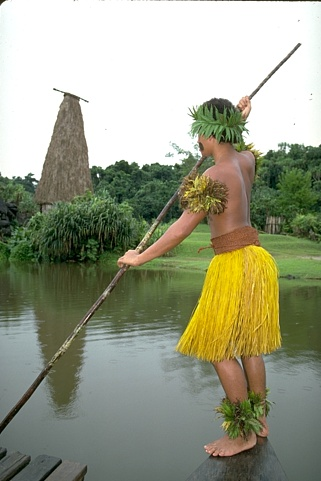
\includegraphics[width=0.3\textwidth]{images/examples/hawaii/arbelaez2011-035.png}
 }
 \subfigure[Edge map]{%
  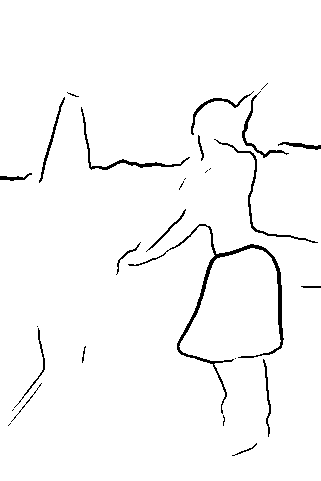
\includegraphics[width=0.3\textwidth]{images/examples/hawaii/edge_map_arbelaez2011-039.png}
  \label{fig:subfigure1}
 }
 \subfigure[Probability of boundary]{%
  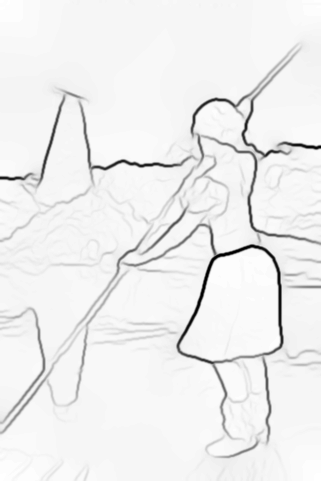
\includegraphics[width=0.3\textwidth]{images/examples/hawaii/Pb_arbelaez2011-039.png}
  \label{fig:subfigure2}
 }
% \quad
% \qquad
% \caption[Caption that doesn't show?]{{\bf Boundary detection} (courtesy~\cite{Arbelaez11}).}
\caption{Referencing subfigure: \protect\subref{fig:subfigure2} some text \protect\subref{fig:subfigure1} some other text}
\label{fig:edge_detection-tryout}
\end{figure}

% simple figure, no labels
\begin{figure}[ht!]
 \centering
 \subfigure[Input image]{%
 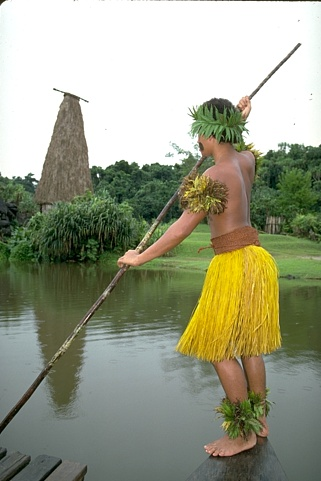
\includegraphics[width=0.3\textwidth]{images/examples/hawaii/arbelaez2011-035.png}
 }
 \subfigure[Edge map]{%
 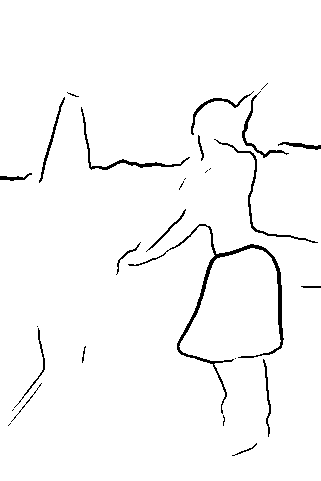
\includegraphics[width=0.3\textwidth]{images/examples/hawaii/edge_map_arbelaez2011-039.png}
 }
\subfigure[Probability of boundary]{%
 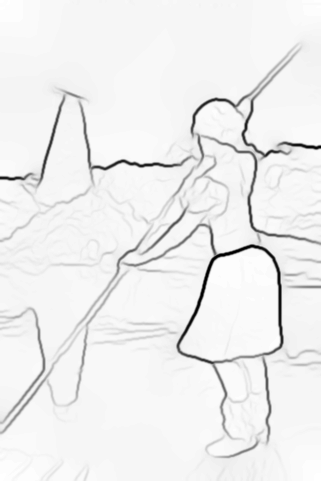
\includegraphics[width=0.3\textwidth]{images/examples/hawaii/Pb_arbelaez2011-039.png}
 }
 \caption[Caption that doesn't show?]{
  {\bf Boundary detection} (courtesy~\cite{Arbelaez11}).}
\end{figure}

\chapter{Introduction}
\label{Chapter1}
\section{Motivation}
\section{Terminology}
\subsection{Edge Detection - Edge, Edge Map, Probability of Boundary}
\subsection{Image Segmentation - Contour, Segmentation, Region Boundary, Hierarchical Segmentation}
\section{Related Work}
% \subsubsection*{Edge Detection}
\subsection{From Edges to Contours}
\subsubsection{Edge Detection}
\subsubsection{Image Segmentation}
\subsection{State-of-the-Art Review}
\section{Outline}
The rest of this work is structured as follows:

% \begin{itemize}
% \item Chapter~\ref{SpectRelax} starts the thesis with a brief introduction to balanced graph cuts and spectral relaxation techniques.
% Section~\ref{sec:ch2_clgrpart} shows that clustering can be seen as a graph partitioning problem. The minimum cut approach often yields useless results where clusters are highly unbalanced, hence
% the balanced graph cut criteria are described in Section~\ref{sec:ch2_balgrcut}.  To solve the NP-hard balanced graph cut problem
% the relaxation methods are applied. Section~\ref{sec:ch2_spectclus} presents the standard spectral clustering approach, which is known to be loose.
% The tight relaxation, called 1-spectral clustering, is described in Section~\ref{sec:ch2_1spectclus}. 
% Section~\ref{ch2:disc} concludes the chapter and discusses the relevance of proposed methods to video segmentation.
% \item Chapter~\ref{chapter3} gives an overview of the video segmentation framework and provides the analysis of low-level features.
% Section~\ref{sec:ch3_framework} introduces the proposed video segmentation model, which employs a two-step approach:
% a graph is constructed on pre-computed superpixels and then a spectral clustering technique is applied. 
% %In graph-based algorithms, in order to produce high-quality segmentation results powerful superpixel similarity measures must be defined.
% Section~\ref{sec:ch3_affinities} gives a description of the graph affinities used in this work.
% To evaluate video segmentation performance and analyze the features of the proposed model we chose the Berkeley motion segmentation dataset, which is presented in Section~\ref{sec:ch3_dataset}.  
% The examination of the quality of the low-level video features is reported in Section~\ref{sec:ch3_aff} and the results are discussed in Section~\ref{ch3:disc}.
% \item Chapter~\ref{Chapter4} provides an experimental comparison of spectral relaxations and analyzes the effects of different balanced graph cuts applied to video segmentation. 
% We start with a brief recap of the main theoretical aspects of 1-norm and 2-norm relaxations in Section~\ref{ch4:recap}.
% Section~\ref{ch4:bench} presents the evaluation benchmark for video segmentation.
% Section~\ref{sec:ch4_1sc_vs_sc} shows the comparison of the performance of spectral clustering and 1-spectral clustering with different balanced graph cut objectives in the task of video segmentation. 
% In order to explore further the balanced cut criteria and the quality of the solutions obtained from the relaxation techniques, we tried to find a better partition by a trivial greedy search optimizing different balanced graph cut functions and see if the ground truth corresponds
% with the minimum cut criterion. The results of the experiments are reported in Section~\ref{sec:ch4_GTexp}.
% Section~\ref{ch4:disc} gives the discussion of the obtained results.
% \item In Chapter~\ref{Chapter5} a methodology for discriminative learning of must-link constraints and their incorporation in the video segmentation framework are proposed.
% Section~\ref{sec:ch5_cosc} shows a way of integrating prior information in the form of must-link constraints into spectral clustering while preserving all the
% balanced graph cuts.
% Section~\ref{sec:llf} presents evaluation of the low-level features as must-link constraints and the connections in the graph based on the ground truth.
% In Section~\ref{sec:ch4_ML} we propose to learn must-links with Random Forest from the affinities.
% We show that even a naive learning approach on the restricted feature space improves video segmentation performance for both relaxations: spectral clustering and 1 spectral clustering. 
% The proposed model is compared to state-of-the-art methods.
% Section~\ref{ch5:disc} discusses the achieved results.
% \item Chapter~\ref{Chapter6} concludes the thesis summarizing all the results of our work and proposing directions for possible improvements.
% \end{itemize}

\chapter{From Edges to Contours - Current State-of-the-Art}
\label{Chapter2}
\section{gPb-owt-ucm Algorithm Pipeline}
\subsection{Quantised Oriented Probability of Boundary}
\subsection{Weighted Watershed}
\section{Flaws of Quantisation}

\chapter{Structured Random Decision Forests}
\label{Chapter3}
\section{Algorithm Outline}
\section{Training - Growing a Decision Forest}
\section{Inference}
\subsection{Sliding Window}
\subsection{Averaging of Overlapping Decisions}

\chapter{Leveraging Structured Forest for Segmentation}
\label{Chapter4}
\section{Edge Detection - gPb vs. Structured Edge}
\section{Weighting the Watershed Locations}
\subsection{Comparing a Structured Forest Patch to a Watershed Patch}
\subsubsection{Patch Transformations}
\subsection{Scoring Functions for Patch Similarity}
\subsubsection{Cast as a Benchmark Problem}
\subsubsection{Boundary and Region Metrics}

\chapter{Experimental Study of Watershed Weighting Strategies}
\label{Chapter5}
\section{Evaluation}
\subsection{Dataset}
\subsection{Metrics}
\section{Exploration of the Space of Weighting Strategies}
\section{Oracle - Experiments with Ground Truth}
\subsection{Oracle Description}
\subsection{Ranking of Oracles}
\subsubsection{Confirms Correct Weighting Strategies}
\subsubsection{Failure Cases}

\chapter{Conclusions and Open Problems}
\label{Chapter6}
\section{Conclusions}
\section{Open Problems}

\clearpage

% TODO double-check the sections hierarchy
% TODO for a $16\times 16$ segmentation patch there exist, in theory $2^256$ possible edge masks. Due to the inherent structure in image patches however, not all of them are likely, and those containing simple structures are prevalent.
\chapter{Capturing image edge structure} %Structured random decision forests}
\label{Chapter2}
In this chapter we discuss the recent edge detection works by Doll\'ar and Zitnick~\cite{DollarICCV13edges,Dollar2015PAMI}. Their algorithm - Structured edge (SE) takes a data-driven approach to learning of semantic edges. % Let the data speak for itself
%Their goal is
They manage to achieve accurate and fast edge detection. % real-time

By ``structure'' in image edges % as well as in SF leaves
we mean the fact that local image patches are known \cite{Ren2006figure,LimZD13} to show % exhibit
notable %prominent
forms of local structure (some examples in Fig.~\ref{fig:srf-structure-in-edge-patches}). As edges are interdependent, often shapes like straight and curved lines, T-junctions and Y-junctions, convexities, sharp corners and parallel lines are to be observed in a local neighbourhood.

\textbf{Capturing more context:} A family of learning approaches have tried to leverage local context to organise images - discover image edges, or recognise %discern
figure from background objects. First the Boosted Edge Learning (BEL) algorithm~\cite{dollar2006supervised} made at each location in the image an independent binary decision as to the presence or absence of image edge. Noticing the abundance of edge structure in a local patch, \textit{sketch tokens}~\cite{LimZD13} and \textit{shapemes}~\cite{Ren2006figure} organise local edge shapes by clustering. The Structured forest (SF)~\cite{DollarICCV13edges} takes this idea a step further and keeps all local segmentation patches it has seen at training time in the leaves of its decision trees. By abstaining from using pre-defined classes of edge patches, clustering, or averaging \textbf{to model local edge context}, the SF framework has the potential to learn subtle variations in edge structure. It is flexible - it is able to adapt to the training dataset at hand by letting the data speak for itself. That is one of the reasons for its highly accurate edge detection.

\textbf{Structured forest ``knows'' image edge context:} Precisely the ability of the structured forest to predict a local segmentation mask given an input image patch is so important to us. Even better, the edge detector SE could provide as a by-product the segmentation predictions that it has made at every image location. We would like to use this information in order to obtain image segmentation.

In this chapter we review the SE edge detector and elucidate why it is a good first-step choice for our task of semantic segmentation.

\section{Structured forests}
\subsection*{Random decision forests}
Random forest (RF) is a recently introduced~\cite{Breiman01} learning approach which has found applications in computer vision~\cite{KontschiederBBP11,LimZD13,DollarICCV13edges,Dollar2015PAMI} due to its speed both at training and testing time, high accuracy, and robustness to noise.

A random decision forest is a collection %an ensemble %a combination 
of tree predictors - classifiers or regressors~\cite{breiman1984classification}. Here ``tree'' is used in the computer science sense to denote an abstract data structure (ADS) - a graph without cycles. 
The predictive power of the forest depends on the strength of the individual trees and their de-correlation. Therefore every tree is constructed based on a vector, sampled independently and randomly from the space of possible vectors. The randomness could be \wrt the training examples that are made available to each tree and\slash or the set of features that are being considered at each node of a decision tree.

Criminisi \etal~\cite{Criminisi12} provide a survey of decision tree methods.

Nowozin~\cite{Nowozin12improvedinformation,nowozin2014decision} discusses bias in the estimation of information gain for making split decisions at each node during decision tree training. He proposes estimators which lead to training better trees, yielding improved predictive performance.

\subsubsection*{Structured learning}
By definition, structured learning means that the input and output spaces can be arbitrarily complex. Examples are images, graphs, strings, bounding boxes, joints positions for object pose estimation, folds of proteins, sequences of actions. The initial methods proposed for the task of structured learning were probabilistic graphical models (PGMs) and structured support vector machines (structured SVMs).

Kontschieder \etal~\cite{KontschiederBBP11} were first to observe that RFs are applicable to the problem of structured learning. They remark that any type of input could be given to RF and they could preserve %conserve 
any type of output in the leaves of the trees. They extend the RF framework to work with structured class labels and use it to perform semantic image labelling (\textit{bike, cow, car, building, road \etc}).

\section{Structured edge algorithm outline}
The key to edge detection using SF is that the decision for a single point is made based on an image patch centred at it. A large enough patch contains low-level features as well as mid-level context information (see Fig.~\ref{fig:srf-structure-in-edge-patches}).

\begin{figure}[ht!]
\centering
 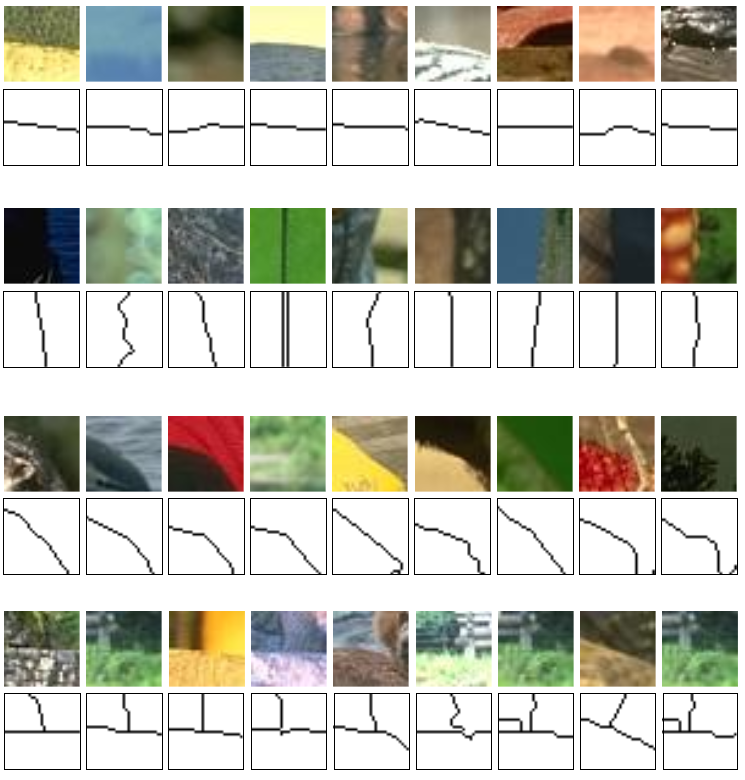
\includegraphics[width=0.3\textwidth]{images/srf/structure-in-edge-patches.png}
\caption{Local edge patches exhibit similar structure. Image patches and the human-%hand-
drawn edges present in them. Cropped from BSDS500, courtesy of~\cite{DollarICCV13PresentationSlides}.}
\label{fig:srf-structure-in-edge-patches}
\end{figure}

SE is an example of supervised machine learning. During training time it is presented with patches and their ground truth annotations (local segmentations). It learns parameters that enable it to make predictions at testing time as to the most likely segmentation of fresh, unseen so far patches. For edge detection, it agglomerates those multiple patch decisions to obtain a probability of boundary (probabilistic edge map) for an entire image.

\section{Training - growing a decision forest}
A RF is trained by recursively growing its decision trees. For the task of edge detection, the training data is a total of 1 million training samples. Half of those are positive examples - a patch containing an edge and its hand-labelled segmentation. The other half are negative examples - so-called ``background patches''. To grow a decision tree means to learn what is a good way of redistributing the input data presented to the tree (at its root node) into its leaves. Such a distribution to the tree leaves would be good if in the end similar training samples are grouped together - in the same decision tree leaf. In the following we discuss binary decision trees, as this is the data structure used in practice by the SE algorithm. It is trivial to extend the algorithm to use general trees by making a multi-class decision at each node. 

% \textbf{Training is redistributing the data towards the leaves of a binary tree:} 
\subsection{Learning the split function}
So at each node a binary decision must be made how to separate the training data into the left and right child sub-trees. Initially the root of the tree contains all training data available to the tree. A split function $h(x,\theta_j)\in\{0,1\}$ determines to which child an input training sample $x$ is forwarded. The parameter $\theta_j$ is what must be learnt for each node $j$ during training. A criterion based on information gain is introduced to decide on optimal %good 
splits. Splitting is done in such a way so as to minimise entropy in the nodes. In this algorithm Gini impurity is used. Some of the improvements proposed by Nowozin~\cite{Nowozin12improvedinformation,nowozin2014decision} regarding entropy estimators are adopted in this work. Growing by splitting a node continues until either 1) a certain maximal tree depth is reached, or 2) sufficient purity of nodes is achieved.

The goal is to cluster in the leaves of the trained structured decision tree segmentation patches that correspond to input features which are as similar as possible. The nett effect is that similar segmentation patches should end up in the same leaf, see Fig.~\ref{fig:structured-decision-tree-node-split}.

\subsection*{Key contribution of the work}
The ``structured output'' in the case of the SE algorithm is a $d\times d$ segmentation patch (in practice they set $d = 16$). 
As the segmentation patch space is high-dimensional and complex, it is non-trivial to compute information gain in order to split the set of inputs into two subsets.

\textbf{Proxy label space:} They introduce a mapping to a simpler, lower-dimensional discrete space. The information gain computed on it is a sufficient approximation of that of the original output space without being prohibitively expensive to compute. Thus it is possible to compute distance, or, analogously, similarity, between output segmentation. In effect, similar output segmentations are clustered together.

\begin{figure}[ht!]
\centering
 \subfigure[A training sample is a pair of image patch and its corresponding ground-truth segmentation.]{%
  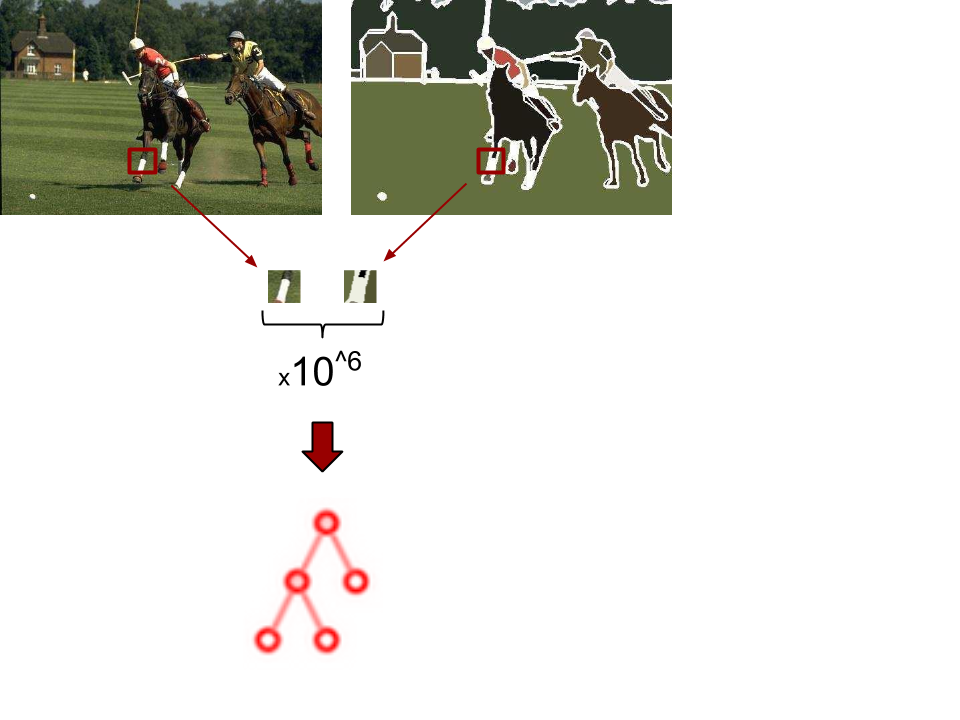
\includegraphics[width=0.5\textwidth]{images/srf/structured-decision-tree-training.png}
 }
 \subfigure[Splitting of training data at a node of a decision tree]{%
  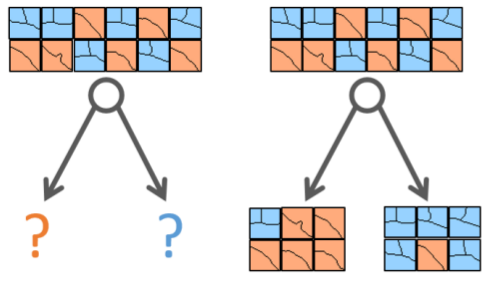
\includegraphics[width=0.3\textwidth]{images/srf/structured-decision-tree-node-split.png}
  \label{fig:structured-decision-tree-node-split}
 }
\caption{Training of a decision tree. \protect\subref{fig:structured-decision-tree-node-split} courtesy of~\cite{DollarICCV13PresentationSlides}.}
\label{fig:srf-training}
\end{figure}

\subsection*{Introducing randomness for diversity of the decision forest}
Part of the accuracy in prediction of the RF framework comes from ensuring sufficient diversity of trees. One way to achieve this, and how it is done in the SE algorithm, is by introducing randomness at each decision node. This is done by subsampling the input features that are taken into account when optimising the split at the tree node. SF achieves robust results by combining the output of $T$ decorrelated trees. Because of the small correlation of the trees in the ensemble, even small forests manage good performance - we later use SE with $T=4$.

\section{Inference}
Unlike other structured learning methods, no optimisation is required to make a prediction. Inference using SF is straightforward. A decision forest is an ensemble of $T$ \textit{independent} trees. To make a prediction, the individual predictions of the trees are combined as prescribed by the ensemble model. Here averaging is performed on the output edge patches.

\subsection{Structured decision tree inference}
The test sample - a feature vector computed based on an input image patch $x$, travels down the tree. Decisions whether it should be routed to the left or right child of a node are made according to the parameters learnt during training. When a leaf node is reached, it contains a set of most likely segmentations, and each of those could be associated with the input $x$.

\textbf{Ensemble model:} In the context of random forests the term ``ensemble model'' defines how to combine multiple predictions into a single prediction. Somewhat confusing, in the paper~\cite{DollarICCV13edges}, this refers to two different things:
\begin{enumerate}
 \item{in decision tree inference:} in order to associate a prediction with the each leaf (like in~\ref{fig:srf-tree-inference}). To this end, the medoid segmentation patch \textit{for the proxy output space} is chosen. This is the one that minimises the sum of distances to all others in the leaf patch, see~\ref{fig:srf-leaf}. The medoid is the only patch that is subsequently used out of all those in the tree leaf. Note that only patches which have been observed during training can be predicted during testing %by the SF
 in this scenario.
 \item{in detection:} to make the final edge detection, a means to combine multiple overlapping decisions is necessary. Details will be given shortly in \textsection~\ref{subsection:edge-detection}.
\end{enumerate}

\begin{figure}[ht!]
\centering
 \subfigure[Image patches used as input, which ended up clustered in the same structured tree leaf.]{%
  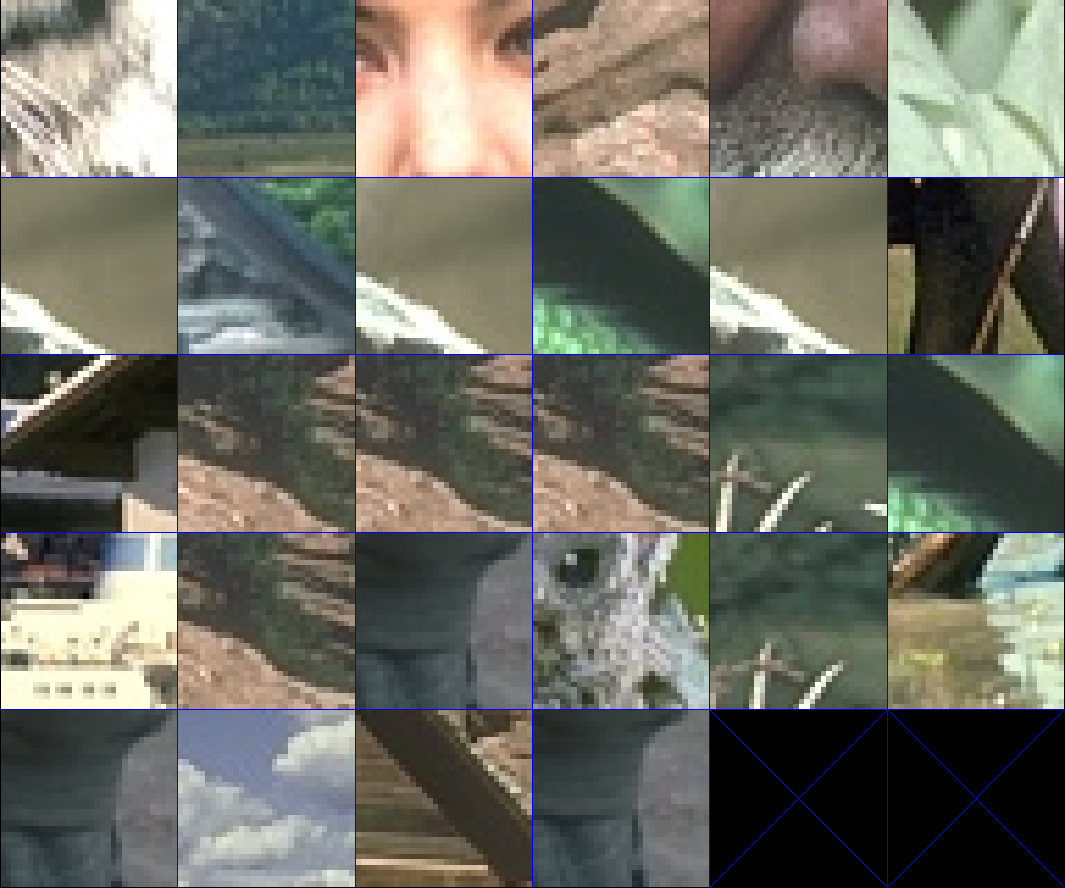
\includegraphics[width=0.45\textwidth]{images/srf/sf-leaf-imgs.png}
  \label{fig:sf-leaf-imgs}
 }
 \subfigure[Corresponding segmentation patches in a structured tree leaf. Upper left is the medoid.]{%
  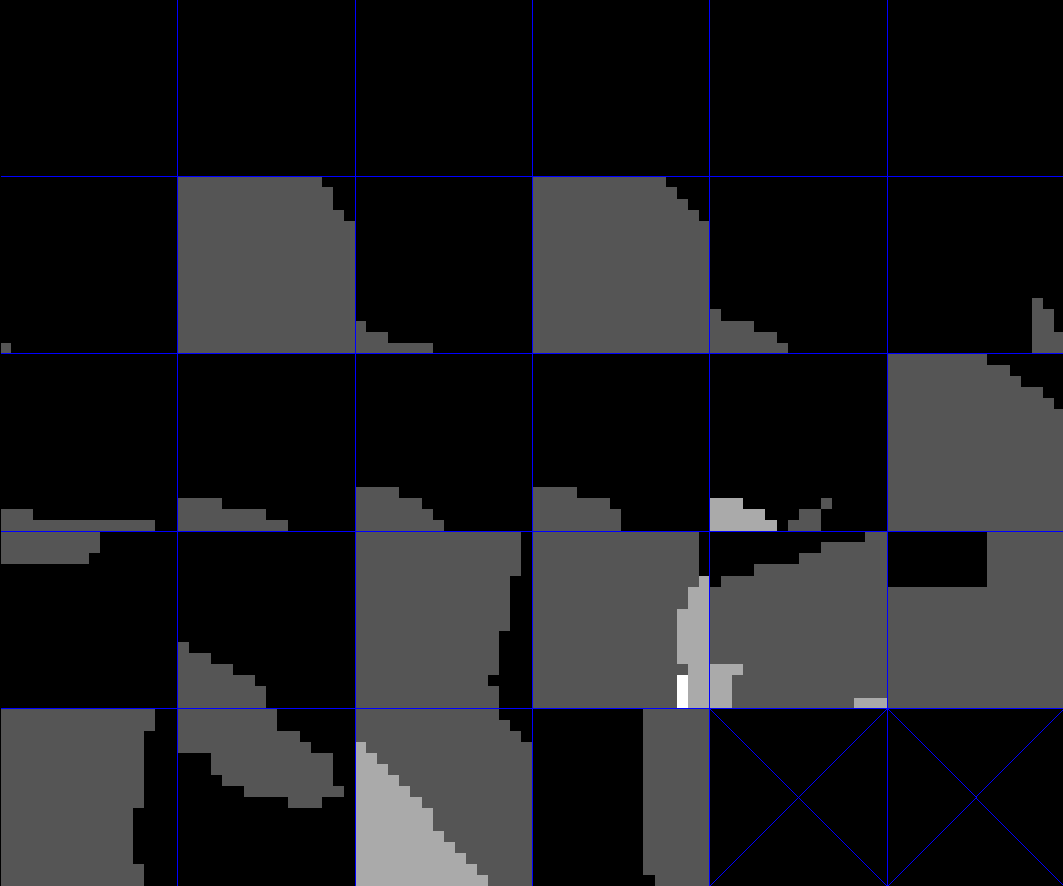
\includegraphics[width=0.45\textwidth]{images/srf/sf-leaf-segs.png}
  \label{fig:sf-leaf-segs}
 }
\caption{Contents of a decision tree leaf. Notice that while the input patches (and consequently, the features computed based on them), are sufficiently similar, the same cannot be said about the segmentation patches. The representative prediction is the medoid - upper left.}
\label{fig:srf-leaf}
\end{figure}

\begin{figure}[ht!]
\centering
 \subfigure[Decision tree inference]{%
  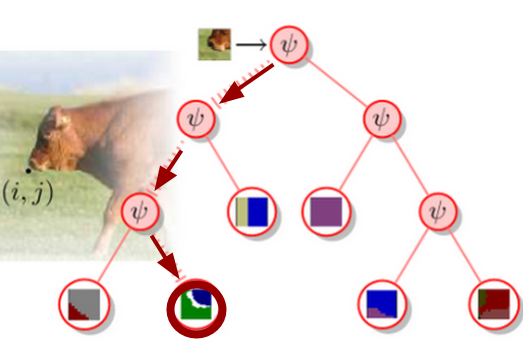
\includegraphics[width=0.57\textwidth]{images/srf/srf-tree-inference.png}
  \label{fig:srf-tree-inference}
 }
 \subfigure[Decision forest as an ensemble of multiple trees]{%
  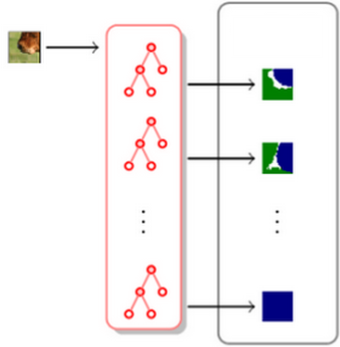
\includegraphics[width=0.4\textwidth]{images/srf/srf-inference-an-ensemble-of-trees.png}
  \label{fig:srf-inference-an-ensemble-of-trees}
 }
\caption{Inference with structured random forest. Images courtesy of~\cite{DollarBlog2013srf}}
\label{fig:srf-inference}
\end{figure}

\subsection{Edge detection}
\label{subsection:edge-detection}
Now that a most-likely segmentation can be obtained given an input image patch, how to do edge detection on a whole image?

\subsubsection*{Sliding window}
Structured labels capture information about entire pixel neighbourhood. Therefore a small number - $T$ of tree predictions per pixel suffice for high edge detection quality. Detection is performed by sliding a window across the image, with a stride $s = 2$, and evaluating, in a chequerboard-pattern a set of $T$ trees. So a total of $2T$ trees are trained. Each of the trees makes a prediction for the given location, many are overlapping. For a patch side of $d = 16$, with $T=4$, each pixel receives $\frac{T*d*d}{s*s}=256$ independent decisions.

\subsubsection*{Averaging of overlapping decisions}
The individual decisions are local segmentation masks. As discussed in \textsection~\ref{Chapter1} it is fairly easy to obtain an edge map, given a segmentation. This is how the multiple patches decisions have to be represented in order to aggregate the information in them for the purposes of edge detection. The combining is done by superimposing, %merging
and then averaging the edge maps from multiple overlapping patches. %decisions. 
This is referred to in the paper~\cite{DollarICCV13edges} as ``custom ensemble model''.

\section{Discussion}
At the time it was published, SE algorithm showed state-of-the-art performance on the now standard benchmark for the task of boundary detection - BPR on BSDS500~\cite{Arbelaez11}. The algorithm is tested on other datasets and the models learnt are capable of successfully finding edges in images from datasets that they were not specifically trained for. This is reassuring - it means that the detector is able to generalise - its knowledge is universal, instead of overly adapted to %fit for 
the contents of a specific dataset.

\subsection*{Alternative way of capturing context}
A different approach is taken by Hallman and Fowlkes in their \textbf{Oriented edge forests (OEF)} paper~\cite{Hallman2014} which was published towards the end of the current research work. They use a decision forest classifier to learn to distinguish between straight-line edges of different position and orientation within an image patch. Although they use a set of pre-defined edge classes, local sharpening of the edges helps them capture fine variations in edge shape. They currently (Feb 2015) achieve best results on the BSDS500 benchmark.

\textbf{OEF for image segmentation:} The output of their algorithm is an oriented probability of boundary $E(x,y,\theta)$. Therefore, it would be a natural fit for the OWT-UCM pipeline described in~\cite{Arbelaez11}. The resulting procedure, which they title ``OEF-OWT-UCM'' allows to use the edge detection results to obtain a hierarchical image segmentation. They report, however, misalignments due to quantisation mismatch of the orientation angles between their algorithm and gPb-OWT-UCM of~\cite{Arbelaez11}.

\subsection*{Strong points of SE}

\begin{itemize}
 \item accurate edge detector,
 \item fast at training time (which is done offline),
 \item real-time speed at test time - during edge detection,
 \item has potential as a general-purpose edge detector, %TODO add note - gPb seems to be highly-tuned for the BSDS500 dataset
 \item is able to predict a most-likely segmentation for a given input patch,
 \item can be augmented to store all those intermediate predictions made during the edge detection.
\end{itemize}


\clearpage

\chapter{From edges to contours} % - Current State-of-the-Art}
\label{Chapter3}
\section{gPb-OWT-UCM algorithm pipeline}


\begin{figure}[ht!]
\centering
 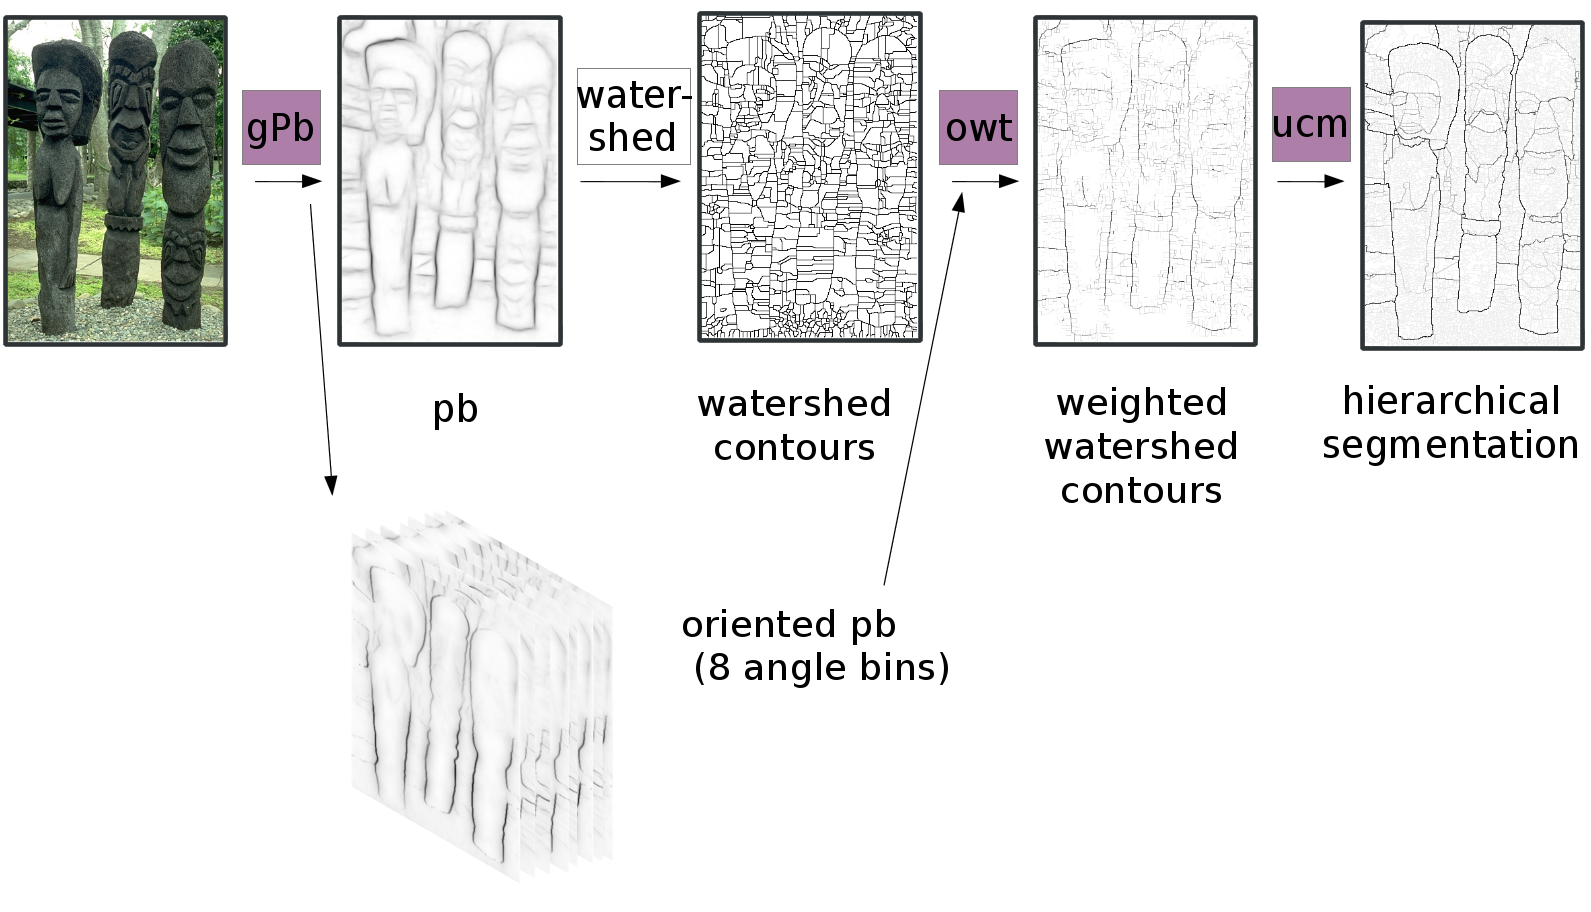
\includegraphics[width=1\textwidth]{images/gPb-OWT-UCM/gPb-OWT-UCM_pipeline.png}
\caption{gPb-OWT-UCM algorithm. We have expanded the pipeline to explicitly include the ``watershed transform'' operation and its output - watershed contours.}
\label{fig:gPb-OWT-UCM-pipeline}
\end{figure}

\subsection{First stage of the pipeline - edge detection} % gPb
The gPb algorithm utilises local cues - colour, brightness and texture to build features. Those are then globalised using spectral clustering. Multiple-scale approach gives competitive edge detection results.
% TODO discuss multiple orientations; put image

\textbf{Quantised oriented probability of boundary}
\subsection{Second stage of the pipeline - weighting the watershed} % OWT
\subsubsection{Watershed}
\label{sec:ch3-watershed}
The watershed transform is a basic morphological operation~\cite{beucher1992morphological} used to produce an image segmentation. Given an intensity %a greyscale 
image as an input, it would output watershed \textit{segments} (\textit{regions}), which are complimentary to the watershed \textit{pixels} (\textit{contours}). The latter are by construction closed contours. A well-known shortcoming of the watershed transform is that the 
segmentation produced by it is an oversegmentation, due to a catchment basin forming around every regional minimum.

Unlike ``Seeded region growing''~\cite{adams1994seeded}, the watershed algorithm does not require as input any initial seeds for forming watershed regions.

Note that the watershed algorithm only provides a single segmentation, but does not build a hierarchy. %but not weights to them, hence, 
Najman~\etal~\cite{najman1996geodesic} offer a way to obtain a hierarchy of segmentations from the watershed pixels, which unfortunatelly involves the selection of a set of markers.

The watershed transform is a suitable intermediate step in obtaining hierarchical segmentation from edge detection output, since it provides a straightforward means to close contours. The probability of boundary is a one-channel image and can therefore be used as an input to the watershed transform. Thus, the locations of the watershed contours constitute a binary image indicating the higest level of recall in the context of the Precision-Recall framework of~\cite{Arbelaez11}. % (c.f. edge map)

In practice the vanilla watershed implementation in MATLAB~\cite{MATLABwatershed} is used, with 8-connected neighbourhood for the regions.

\subsubsection*{Oriented watershed transform (OWT)}
\label{sec:ch3-OWT}
% TODO define watershed arcs

\subsection{Third stage of the pipeline - UCM}
\label{sec:ch3-UCM}
% coarse-to-fine
% agglomerative clustering

\section{Limitations of the gPb-OWT-UCM} %quantisation} % or drawbacks, don't say 'flaws'
Quantisation
\clearpage

\chapter{Leveraging structured forest for segmentation}
\label{Chapter4}
Given an edge detection result, various methods could be employed to obtain image segmentation.  One approach is to try and identify all possible boundaries of segmentation regions, based on the probability of boundary score produced by the edge detector. Those boundaries %, called \textit{watershed pixels}, 
finely partition the image pixel graph (see \textsection~\ref{sec:ch3-watershed} for a description of the \textit{watershed transform} which we will use). The regions closed by them constitute an oversegmentation of the image. Different tasks require segmentation at different level of detail. It is useful, therefore, to be able to obtain coarser segmentations as well. 
By reasoning about the salience of region boundaries, one could construct a \textit{hierarchy of segmentations} (see \textsection~\ref{sec:ch3-UCM} for details on the UCM). Going up the hierarchy corresponds to coarsening the segmentation by merging neighbouring regions which are separated by a weak boundary. To establish the order in which to merge the regions, we must be able to tell weak from strong boundaries. We want to associate a \textit{score} with every possible region boundary, which score should reflect the strength of that intervening boundary.

\textbf{Structured voting:} To score the region boundaries we take a patch comparison approach. The edge detector which we employ, Structured edge (SE) by Doll\'ar~\etal~\cite{DollarICCV13edges}, associates a segmentation to every patch centred around a pixel location in the image - its most likely segmentation. The possible region boundaries locations are obtained by a watershed transformation on the output of this detector. For the same location we attain a patch from the watershed locations image. We then explore strategies to compare those two patches and score the similarity between them, a higher score meaning higher local evidence for boundary. We call those \textbf{watershed weighting strategies}. The choice of such an approach defines how we conduct our \textbf{Structured voting (SV)}.

\textbf{How to vote? Two essentials:} We identify two important points in order to be able to score the two patches just described. 
Firstly, one being a local segmentation, and the other - a local oversegmentation, they are quite dissimilar. Therefore, one patch needs to be sensibly \textbf{transformed}, so that the two patches are comparable. 
Secondly, given that the two patches are comparable, what \textbf{scoring function} should be employed? We cast the problem of comparing two segmentation patches as a segmentation benchmark problem. Various boundary- and region-based metrics have been proposed for the task of evaluating image segmentation. We analyse the theoretical properties of some, and use a suitable %reasonable 
subset of them in our practical experiments. 
So a watershed weighting strategy has two aspects - making the patches sufficiently similar to compare, and choosing a scoring function to compare them.

\textbf{Pipeline:} In the terms of the framework of Arbel\'aez~\etal~\cite{Arbelaez11} - gPb-OWT-UCM, we propose to use SE instead of gPb as an edge detector. Further, we replace the Oriented watershed transform (OWT) by SV to obtain scored region boundary locations. Our image segmentation pipeline could then be titled \textbf{SE-SV-UCM}, see Fig.~\ref{fig:SE-SV-UCM-pipeline}.

\begin{figure}[ht!]
\centering
 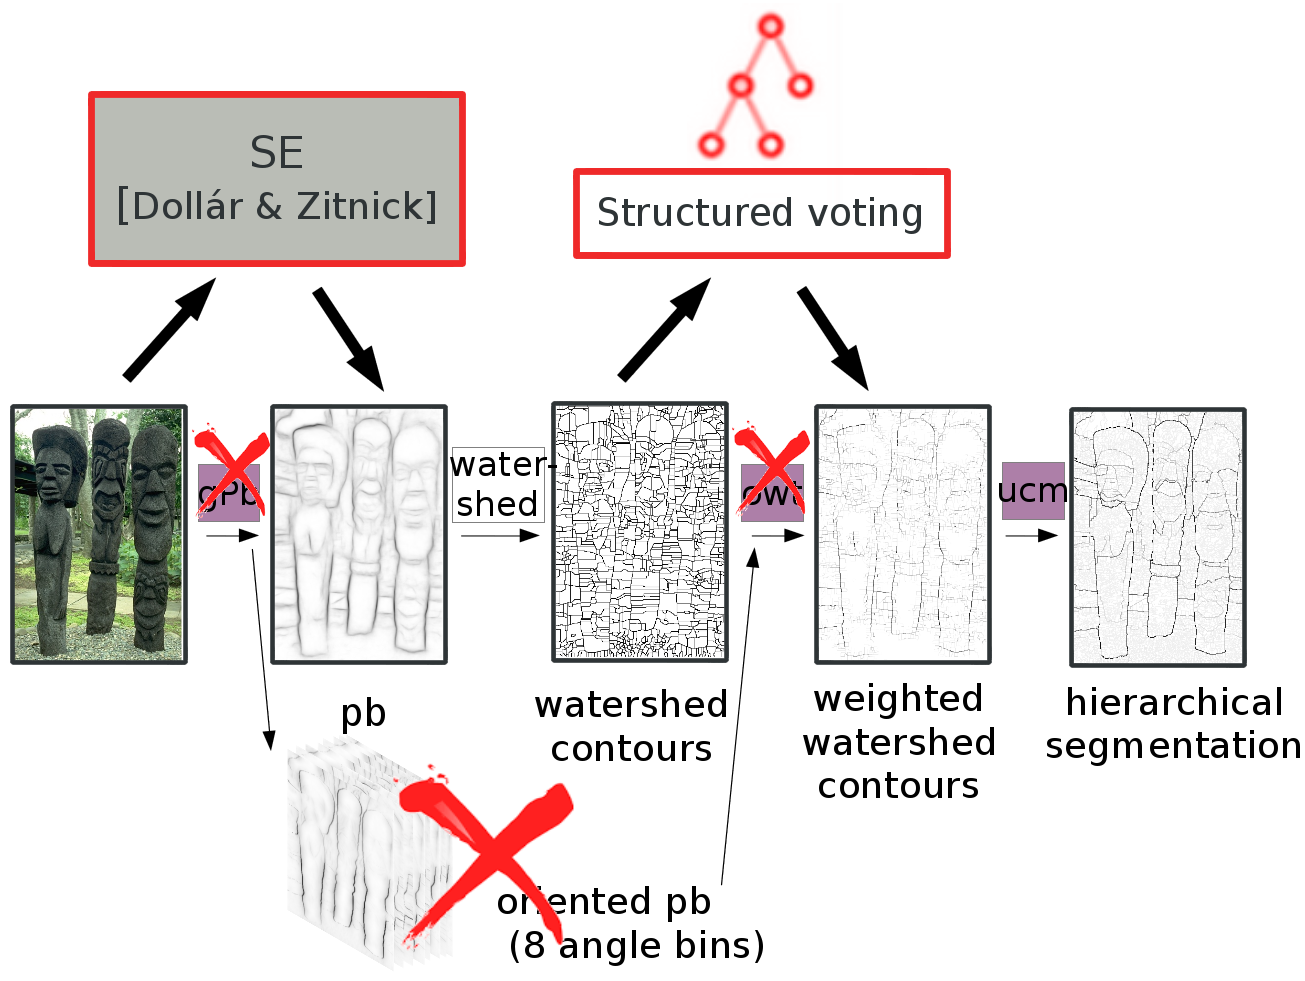
\includegraphics[width=1\textwidth]{images/SE-SV-UCM/SE-SV-UCM_pipeline.png}
\caption{Our SE-SV-UCM algorithm in the context of gPb-OWT-UCM pipeline, see Fig.~\protect\ref{fig:gPb-OWT-UCM-pipeline}.}
\label{fig:SE-SV-UCM-pipeline}
\end{figure}

In the rest of the chapter we describe our algorithm's pipeline. We finish with a discussion on practical issues concerning edge detection and image segmentation output format.

\section[First stage of the pipeline - Structured edge]{First stage of the pipeline - edge detection - Structured edge}
We employ the edge detector SE of~\cite{DollarICCV13edges,Dollar2015PAMI}.

\subsection{gPb vs. SE}
The gPb algorithm uses a combination of carefully designed features - the gradients, each at 3 scales of: 1) texture, 2) brightness, and 3) color (a total of 9 channels). As Doll\'ar reports in~\cite{DollarICCV13edges}, despite a high score on the BSDS500 dataset, gPb performs poorly when tested on other datasets. This is potentially a symptom of over-tuning of the algorithm to the dataset.

Beside being heavily-engineered, in terms of detection speed it does not come close to the real-time performance of SE.

The chief reason for using SE for us, however, is that this edge detector can provide as a by-product the intermediate most likely-segmentations that it has predicted per location in the image. This is important information about the local edge structure that we will build on when developing our Structured voting.

\section{Second stage of the pipeline - Structured voting}
\label{sec:ch4-SE-SV-UCM_SV_details}
The goal of SV is to propose a suitable way of associating a score with each of the watershed pixel. Inspired by the ``local patch as a means of capturing context'' philosophy of previous works~\cite{dollar2006supervised,LimZD13,DollarICCV13edges}, we take a patch comparison approach.

\subsection{Weighting the watershed contours} %locations}
\textbf{Casting a single vote:} The SE provides us ``for free'' with the best segmentation patches - local decisions that the trees of the decision forest have made on all locations of the image. We crop, centred around the same location, a patch of the same size ($16\times 16$ pixels) from the watershed superpixels  image. Comparing the two gives us a score, which we associate with the location on the watershed contours.

\textbf{Votes averaging:} A total number of $T=4$ votes are cast per watershed pixel, and we take the mean of those. To further denoise the voting and give our votes a larger platform, % stage, dais, rostrum, podium
we average all votes per \textit{watershed arc}. The watershed arcs, as discussed in~\ref{sec:ch3-OWT}, are edges of the watershed contours, which are fairly consistent in their orientation. They are obtained by recursively subdividing the region boundaries of the watershed until the approximation given by the straight line through the end of the watershed arc is a sufficiently good one. % TODO artifact from the OWT

\subsection{Comparing a structured forest patch to a watershed patch}
\begin{figure}[ht!]
\centering
 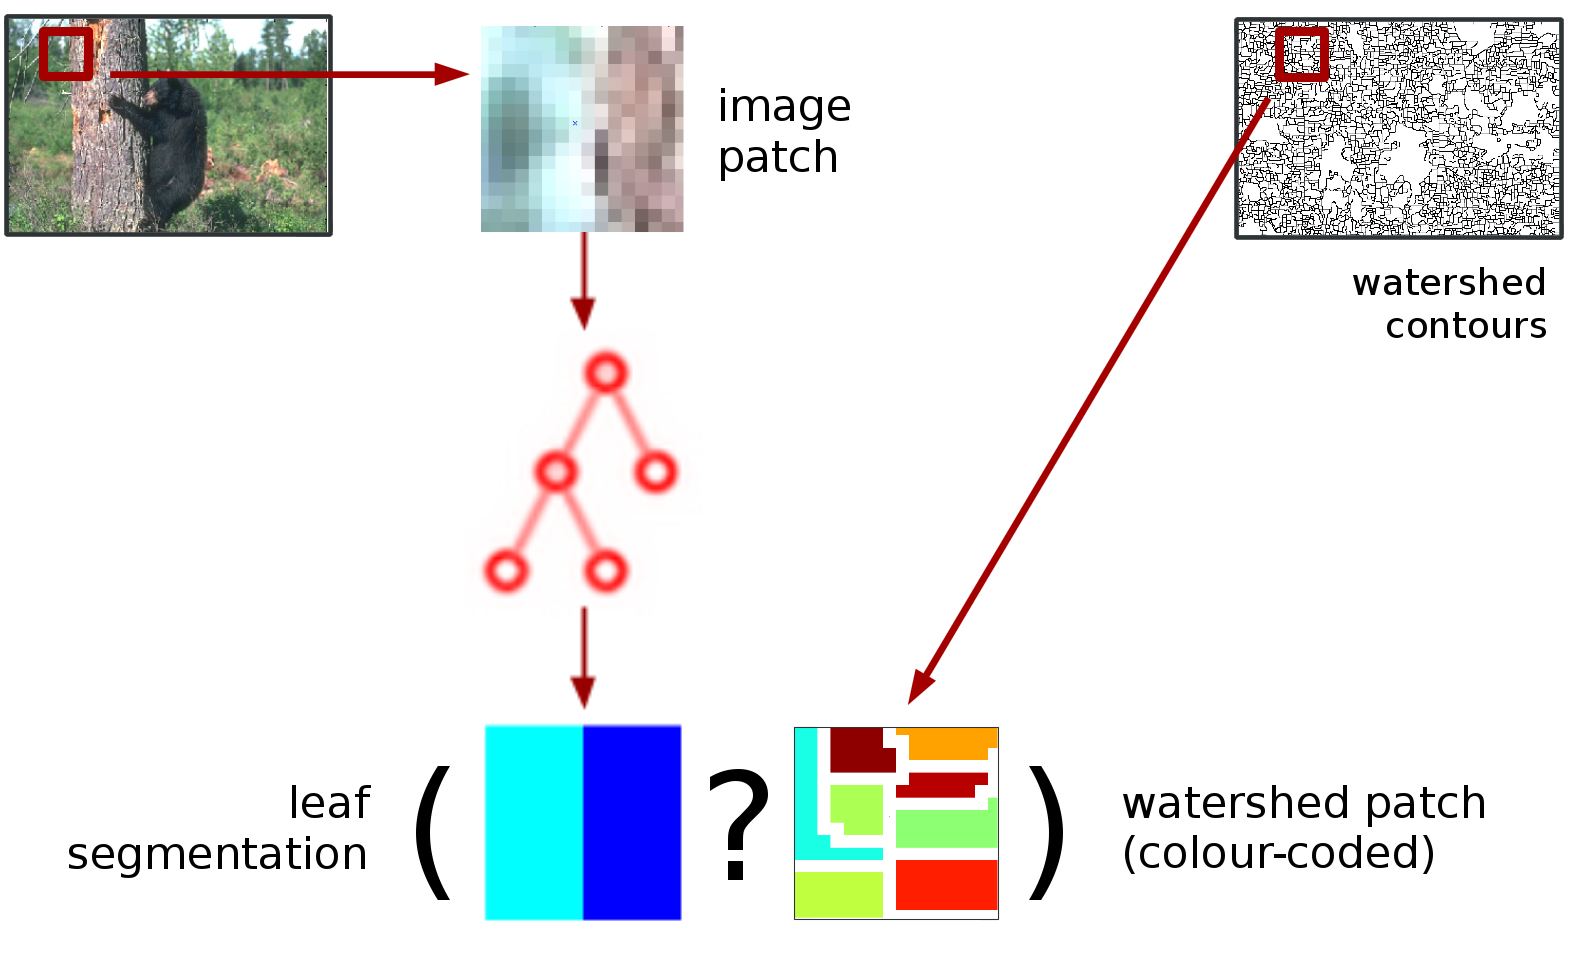
\includegraphics[width=1\textwidth]{images/SE-SV-UCM/weighting-the-watershed-contours-two-patches.png}
\caption{We have the task of comparing and scoring the similarity of two patches - a \textbf{decision tree leaf segmentation} and a \textbf{watershed oversegmentation}.}
\label{fig:weighting-the-watershed-contours}
\end{figure}

For a specific location one tree of the structured forest predicts a segmentation. From the watershed we have a corresponding patch, see fig.~\ref{fig:weighting-the-watershed-contours}. As mentioned already, there are two aspects to scoring their similarity: 1) making them suitable (\ie sufficiently similar) for comparison, and 2) choosing a function that can assess the agreement between the two patches as to the presence or absence of an edge.

\subsubsection{Patch transformations}
To appreciate the necessity of making the two types of segmentation patches comaprable, look at fig.~\ref{fig:watershed-and-leaf-patches}.

\textbf{Watershed patch:} The watershed patch is an oversegmentation with an \textbf{explicit boundary of size 1 pixel} between the segments.

\textbf{Tree leaf patch:} The segmentation patches from the Structured forest are the learnt best segmentation for the given location in the image (based on the features computed from a cropped image patch). They are patches ``seen'' by the forest during the training phase. Since the SE algorithm uses \textbf{supervised learning}, the patches are cropped from the ground truth annotated segmentations. 
For the BSDS500 the segmentation labels  are assigned by humans, and they are never oversegmentations (fig.~\ref{fig:BSDS-annotations} has an example image and its annotations). 
For a $16\times 16$ pixels local segmentation patch there rarely are more than \textbf{2 or 3 segments}. 
A ground truth segmentation in this dataset constitutes a labelling of the pixels, so that homogenous regions - superpixels, are formed. The labels are unique and the \textbf{boundary between segments is implicit}.
Note that in~\ref{fig:watershed-and-leaf-patches} we only show examples of \textbf{non-background} patches. Background patches would contain a single region - the whole patch. Clearly, %Evidently, 
they present local evidence of lack of boundary.

\begin{figure}[ht!]
\begin{center}
  \begin{tabular}{ cccccc }
  
\includegraphics[width=0.13\textwidth,frame]{images/SE-SV-UCM/watershed-patches/watershed-patch1.png} &  
\includegraphics[width=0.13\textwidth,frame]{images/SE-SV-UCM/watershed-patches/watershed-patch2.png} &
  
\includegraphics[width=0.13\textwidth,frame]{images/SE-SV-UCM/watershed-patches/watershed-patch3.png} &
  
\includegraphics[width=0.13\textwidth,frame]{images/SE-SV-UCM/leaf-patches/leaf-patch2.png} & % 
\includegraphics[width=0.13\textwidth,frame]{images/SE-SV-UCM/leaf-patches/leaf-patch1.png} & % too similar to leaf-patch4.png
  
\includegraphics[width=0.13\textwidth,frame]{images/SE-SV-UCM/leaf-patches/leaf-patch13.png} &
  
\includegraphics[width=0.13\textwidth,frame]{images/SE-SV-UCM/leaf-patches/leaf-patch4.png} \\

  
\includegraphics[width=0.13\textwidth,frame]{images/SE-SV-UCM/watershed-patches/watershed-patch4.png} &
  
\includegraphics[width=0.13\textwidth,frame]{images/SE-SV-UCM/watershed-patches/watershed-patch5.png} &
  
\includegraphics[width=0.13\textwidth,frame]{images/SE-SV-UCM/watershed-patches/watershed-patch6.png} &
  
\includegraphics[width=0.13\textwidth,frame]{images/SE-SV-UCM/leaf-patches/leaf-patch3.png} &
  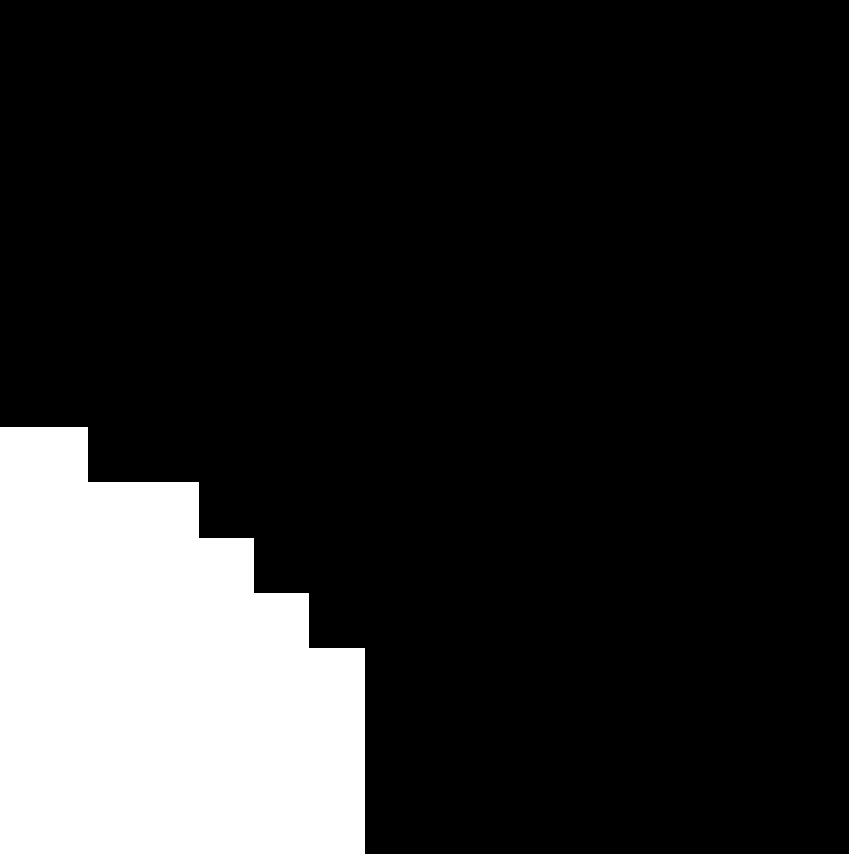
\includegraphics[width=0.13\textwidth,frame]{images/SE-SV-UCM/leaf-patches/leaf-patch5.png} &
  
\includegraphics[width=0.13\textwidth,frame]{images/SE-SV-UCM/leaf-patches/leaf-patch6.png} \\

  
\includegraphics[width=0.13\textwidth,frame]{images/SE-SV-UCM/watershed-patches/watershed-patch9.png} &
  
\includegraphics[width=0.13\textwidth,frame]{images/SE-SV-UCM/watershed-patches/watershed-patch7.png} &
  
\includegraphics[width=0.13\textwidth,frame]{images/SE-SV-UCM/watershed-patches/watershed-patch8.png} &
  
\includegraphics[width=0.13\textwidth,frame]{images/SE-SV-UCM/leaf-patches/leaf-patch7.png} &
  
\includegraphics[width=0.13\textwidth,frame]{images/SE-SV-UCM/leaf-patches/leaf-patch8.png} & % 
\includegraphics[width=0.13\textwidth,frame]{images/SE-SV-UCM/leaf-patches/leaf-patch9.png} \\ % too similar to leaf-patch8.png
  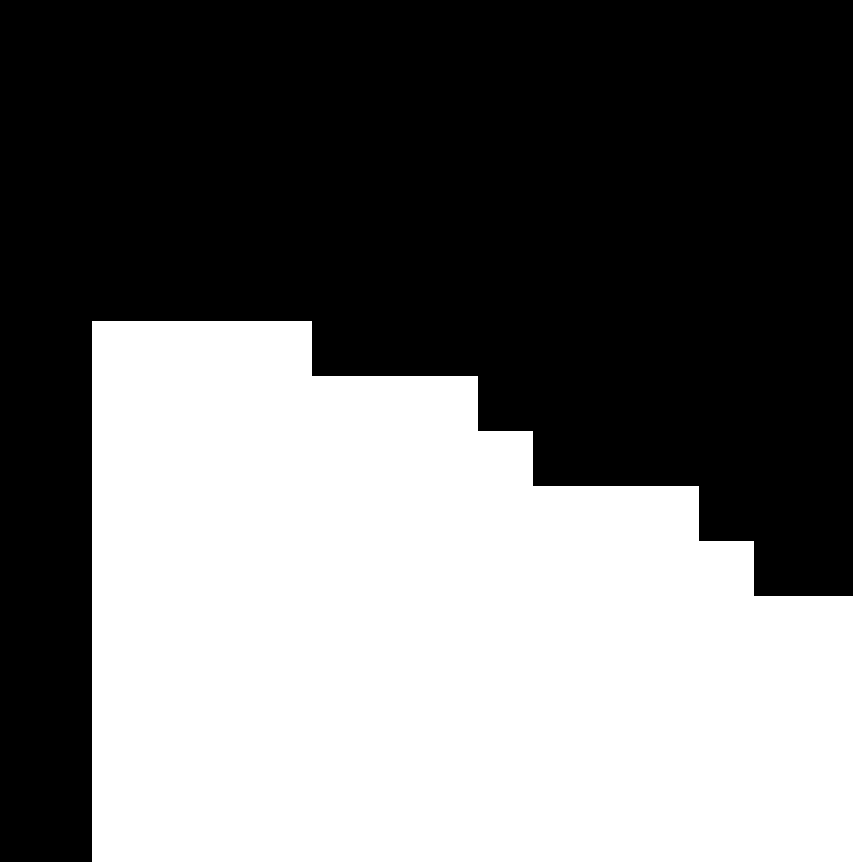
\includegraphics[width=0.13\textwidth,frame]{images/SE-SV-UCM/leaf-patches/leaf-patch18.png} \\

  
\includegraphics[width=0.13\textwidth,frame]{images/SE-SV-UCM/watershed-patches/watershed-patch10.png} &
  
\includegraphics[width=0.13\textwidth,frame]{images/SE-SV-UCM/watershed-patches/watershed-patch11.png} &
  
\includegraphics[width=0.13\textwidth,frame]{images/SE-SV-UCM/watershed-patches/watershed-patch12.png} &
  
\includegraphics[width=0.13\textwidth,frame]{images/SE-SV-UCM/leaf-patches/leaf-patch10.png} &
  
\includegraphics[width=0.13\textwidth,frame]{images/SE-SV-UCM/leaf-patches/leaf-patch11.png} &
  
\includegraphics[width=0.13\textwidth,frame]{images/SE-SV-UCM/leaf-patches/leaf-patch12.png} \\

  
\includegraphics[width=0.13\textwidth,frame]{images/SE-SV-UCM/watershed-patches/watershed-patch13.png} &
  
\includegraphics[width=0.13\textwidth,frame]{images/SE-SV-UCM/watershed-patches/watershed-patch14.png} &
  
\includegraphics[width=0.13\textwidth,frame]{images/SE-SV-UCM/watershed-patches/watershed-patch15.png} &
  
\includegraphics[width=0.13\textwidth,frame]{images/SE-SV-UCM/leaf-patches/leaf-patch-3-segms1.png} &
  
\includegraphics[width=0.13\textwidth,frame]{images/SE-SV-UCM/leaf-patches/leaf-patch-3-segms2.png} &
  
\includegraphics[width=0.13\textwidth,frame]{images/SE-SV-UCM/leaf-patches/leaf-patch-3-segms3.png} \\
  \end{tabular}
  % unused watershed patches: watershed-patch 16 17
  %
  % unused leaf patches: leaf-patch 1 9 14 15 16 17
  %                      leaf-patch-3-segms 4 5 6 7 
  % leaf-patch-_maybe_problematic - two separate segments with the same label % do we handle that? hmmm....
\end{center}
\caption{Examples of \textbf{watershed} patch segmentations (colour-coded on the \textbf{left}; white pixels mark the explicit boundary) and structured decision \textbf{tree leaf} patch segmentations (greyscale on the \textbf{right}).}
\label{fig:watershed-and-leaf-patches}
\end{figure}

\paragraph{Greedy merge}\mbox{}\\\mbox{}\\ % force some space after the paragraph name
For this paragraph, please first have a look at fig.~\ref{fig:ws-greedy-merge}. Evidently merely converting the watershed oversegmentation to have implicit boundaries (from the original watershed patch segmentation - fig.~\ref{fig:sub:watershed-colour-coded} to the segmentation labelling - fig.~\ref{fig:sub:watershed-segments}) is not sufficient. The watershed is still very different from the target - the decision tree leaf patch (fig.~\ref{fig:sub:tree-leaf}), in the sense that it contains many more segments.

\textbf{Na\"{\i}ve greedy merge:} Our first attempt, which we call na\"{\i}ve greedy merge, suffered from the limitation of being overly 
greedy. The transformed watershed patch (see fig.
~\ref{fig:sub:watershed-naive-greedy-merge}) adapts itself excessively to the tree leaf segmentation which we use to guide the merging. As a consequence, it does not respect the fact that the watershed patch has a boundary pixel in the middle, hence, there must be no less than two segments abutting its centre pixel.

\textbf{Fair greedy merge:} As a remedy, we propose a ``fairer'' greedy merge. It %uses heuristic to
aims for an optimal superpixels merge into segments, according to the structured tree patch (fig.~\ref{fig:sub:tree-leaf}). At the same time it still respects the condition that the central watershed pixel lies on a boundary between two regions. Fig.~\ref{fig:sub:watershed-fairer-greedy-merge} shows an example.

\begin{figure}[ht!]
\centering
 \subfigure[Input image]{%
  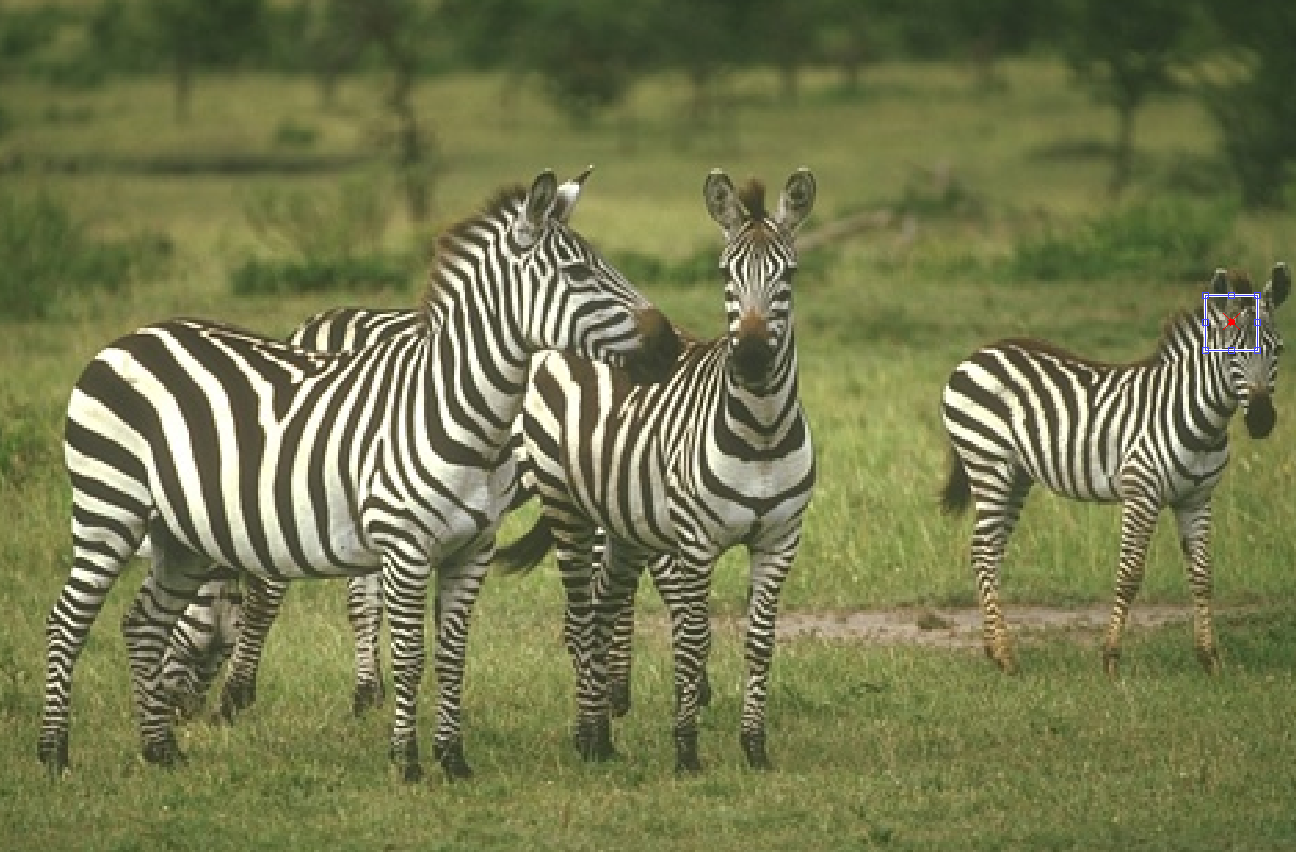
\includegraphics[width=0.5\textwidth]{images/SE-SV-UCM/ws-greedy-merge/zebras2.png}
 }
 \subfigure[Cropped image patch]{%
  
\includegraphics[width=0.2\textwidth]{images/SE-SV-UCM/ws-greedy-merge/selected-image-patch.png}
 }

 \subfigure[Cropped watershed patch]{%
  \includegraphics[width=0.2\textwidth,frame]{images/SE-SV-UCM/ws-greedy-merge/watershed-colour-coded.png}
  \label{fig:sub:watershed-colour-coded}
 }
 \subfigure[Watershed patch with implicit region boundaries]{%
  \includegraphics[width=0.2\textwidth,frame]{images/SE-SV-UCM/ws-greedy-merge/watershed-segments.png}
  \label{fig:sub:watershed-segments}
 } \qquad\qquad\qquad\qquad\qquad

 \subfigure[Tree leaf segmentation patch that guides the merging]{%
  \includegraphics[width=0.2\textwidth,frame]{images/SE-SV-UCM/ws-greedy-merge/tree-leaf.png}
  \label{fig:sub:tree-leaf}
 }
 \subfigure[Watershed patch {\bf na\"{\i}ve} greedy merge]{%
  \includegraphics[width=0.2\textwidth,frame]{images/SE-SV-UCM/ws-greedy-merge/watershed-naive-greedy-merge.png}
  \label{fig:sub:watershed-naive-greedy-merge}
 }
 \subfigure[Watershed patch {\bf fair} greedy merge]{%
  \includegraphics[width=0.2\textwidth,frame]{images/SE-SV-UCM/ws-greedy-merge/watershed-fairer-greedy-merge.png}
  \label{fig:sub:watershed-fairer-greedy-merge}
 }
\caption[{\bf Greedy merge} of watershed patch.]{{\bf Greedy merge} of watershed patch. The central pixel of the patches is marked, as it is important, see the text for details.}
\label{fig:ws-greedy-merge}
\end{figure}

\paragraph{Watershed arc}\mbox{}\\\mbox{}\\ % previously called ``just contour'' % region boundary
Watershed

\begin{figure}[ht!]
\begin{center}
 \subfigure[Input image]{%
  \includegraphics[width=0.14\textwidth]{images/SE-SV-UCM/ws-just-contour/old_man.png}
 }
 \subfigure[Cropped image patch]{%
  \includegraphics[width=0.15\textwidth]{images/SE-SV-UCM/ws-just-contour/selected-image-patch.png}
 }
 \subfigure[Matching %Corresponding 
 watershed patch]{%
  \includegraphics[width=0.15\textwidth,frame]{images/SE-SV-UCM/ws-just-contour/watershed-colour-coded.png}
  \label{fig:sub:ws-just-contour-watershed-colour-coded}
 }
 \subfigure[\protect\subref{fig:sub:ws-just-contour-watershed-colour-coded}~transformed - just an arc]{%
  \includegraphics[width=0.15\textwidth,frame]{images/SE-SV-UCM/ws-just-contour/watershed-just-contour.png}
  \label{fig:sub:ws-just-contour-watershed-just-contour}
 }

 % for the next 8 images, wisth=0.15 also works
 \subfigure[The 4 tree leaf segmentations]{%
  \begin{tabular}{ cccc }
  Tree 1 & Tree 2 & Tree 3 & Tree 4 \\
  \includegraphics[width=0.13\textwidth,frame]{images/SE-SV-UCM/ws-just-contour/tree1-seg.png} &
  \includegraphics[width=0.13\textwidth,frame]{images/SE-SV-UCM/ws-just-contour/tree2-seg.png} &
  \includegraphics[width=0.13\textwidth,frame]{images/SE-SV-UCM/ws-just-contour/tree3-seg.png} &
  \includegraphics[width=0.13\textwidth,frame]{images/SE-SV-UCM/ws-just-contour/tree4-seg.png} \\
  \end{tabular}
  \label{fig:sub:tree-leaf-segments}
 }

 \subfigure[\protect\subref{fig:sub:tree-leaf-segments}~transformed to boundaries]{
  \begin{tabular}{ cccc }
  \includegraphics[width=0.13\textwidth,frame]{images/SE-SV-UCM/ws-just-contour/tree1-bdry.png} &
  \includegraphics[width=0.13\textwidth,frame]{images/SE-SV-UCM/ws-just-contour/tree2-bdry.png} &
  \includegraphics[width=0.13\textwidth,frame]{images/SE-SV-UCM/ws-just-contour/tree3-bdry.png} &
  \includegraphics[width=0.13\textwidth,frame]{images/SE-SV-UCM/ws-just-contour/tree4-bdry.png} \\
  \end{tabular}
  \label{fig:sub:tree-leaf-boundaries}
  }
\end{center}
\caption[Watershed transformation to just {\bf region boundary}]{Watershed transformation to just {\bf region boundary}.}
\label{fig:watershed-just-contour}
\end{figure}

\paragraph{Line fitting}\mbox{}\\\mbox{}\\
Line

\paragraph{Quadratic fitting}\mbox{}\\\mbox{}\\
Quadratic

\subsection{Scoring functions for patch similarity}
We cast the problem of scoring the similarity of a watershed and a structured tree leaf patch as a segmentation benchmark problem. To this end we review some popular boundary and region metrics proposed for the task and see what are the challenges in using them as scoring functions in our scenario.

\subsubsection{Boundary and region metrics}
\label{sec:ch4-boundary-and-region-metrics-maths}
In the following we will use $S$ to denote machine boundary map, $\mathbb{S}$ for machine segmentation, $s$ for a segment in it, $G$ for a ground-truth boundary map, $\mathbb{G}$ for ground-truth segmentation, and $g$ for a segment in it.

\paragraph{Boundary Precision-Recall (BPR)}\mbox{}\\\mbox{}\\
The metric was proposed by~\cite{Arbelaez11} to evaluate the quality of edge detection algorithms in a precision-recall framework. Precision measures the fraction of true positive edge pixels. Recall evaluates the amount of real (\eg ground-truth-annotated) edge pixels detected by the algorithm under test. The reported measure is the \textbf{F-score}, which is the harmonic mean of the precision and recall.

\label{sec:ch4-BPR-maths}
\[
P=\frac{\left|S\cap\left(\bigcup\limits _{i=1}^{M}G_{i}\right)\right|}{|S|}
\]
\[
R=\frac{{\sum\limits _{i=1}^{M}\left|S\cap G_{i}\right|}}{\sum\limits _{i=1}^{M}\left|G_{i}\right|}
\]
\[
F=\frac{2PR}{P+R}
\]

where $S$ and $\{G_{i}\}_{i=1}^{M}$ are boundary maps and $\cap$
computes a bipartite graph assignment between them.

\paragraph{Rand index (RI)}\mbox{}\\\mbox{}\\
Rand index, or Rand measure~\cite{rand1971objective} is a statistical measure of the similarity between two data clusters.

\subparagraph*{Rand index (RI)}\mbox{}\\
Here is how the RI between two segmentations could be defined.

\begin{align*}
RI(S,G) & =\frac{1}{T}\sum\limits _{j<k}\left[\mathbb{I}\left(S(j)=S(k)\wedge G(j)=G(k)\right)+\mathbb{I}\left(S(j)\neq S(k)\wedge G(j)\neq G(k)\right)\right]\\
 & =\frac{1}{T}\sum\limits _{(j,k)\in A}\left[c_{jk}\mathbb{I}\left(G(j)=G(k)\right)+(1-c_{jk})\mathbb{I}\left(G(j)\neq G(k)\right)\right]
\end{align*}

where $\mathbb{I}$ - the identity function,

$S(j)$ - the label of pixel $j$ in the segmentation $S$,

$c_{jk}=\mathbb{I}\left(S(j)=S(k)\right)$ - the event of the pair
of pixels $j$ and $k$ having the same label in segmentation $S$,

$A=\{(j,k)|j<k\}$ - the set of unique pairs of pixels,

$N=\left|S\right|=\left|G\right|$ - the number of pixels in the image
(and each segmentation); in our case with $16\times 16$ patches, $N=16 . 16 = 256$, and 

$T=|A|=\binom{N}{2}$ - the number of possible unique pairs among
$N$ pixels; for us - $\binom{16 . 16}{2}=32 640$.


\subparagraph*{Rand Index Monte Carlo (RIMC)}\mbox{}\\ %RSRI (Random Subsample RI)} previously CPD (Crude Patch Distance), which was a misnomer
\label{sec:ch4-RIMC-maths}
The RIMC is different from RI in that it takes a Monte Carlo subsample of the possible unique pairs of pixels and only considers their segment membership. It is inspired by the implementation of randomised label mapping to a simpler discrete space in training nodes of a decision forests in~\cite{DollarICCV13edges}. We define the RIMC between two segmentations.

\[
RIMC(S,G)=\frac{1}{T}\sum\limits _{(j,k)\in B}\left[c_{jk}\mathbb{I}\left(G(j)=G(k)\right)+(1-c_{jk})\mathbb{I}\left(G(j)\neq G(k)\right)\right]
\]

where $B\subsetneq A$ - a random subset of the pairs of pixels.
In our experiments $|B|=256$.


\subparagraph*{Probabilistic Rand index (PRI)}\mbox{}\\
Probabilistic Rand index~\cite{UnnikrishnanPH07} counts the number of pixel pairs with agreement in %consistent 
labelling between a machine generated segmentation on one hand, and \textbf{multiple} ground truth segmentations on the other hand.

% between a test segmentation and multiple ground truths

\[
PRI(S,\{G_{i}\}_{i=1}^{M})=\frac{1}{T}\sum\limits _{j<k}\left[c_{jk}p_{jk}+\left(1-c_{jk}\right)\left(1-p_{jk}\right)\right]
\]


where $p_{jk}$ - probability of $c_{jk}$; possible estimator of
$p_{jk}$ is the sample mean of the corresponding Bernoulli distribution.


\paragraph{Segmentation covering (SC)}\mbox{}\\\mbox{}\\
To be able to understand Segmentation covering and Volume Precision-Recall, which we define in the next paragraph, it is helpful to first have a notion of the related \textit{Overlap} and \textit{Intersection over union}.

\subparagraph*{Overlap, or Jaccard index}\mbox{}\\
Overlap of two regions % segments
$s$ and $g$

\[
\mathcal{O}\left(s,g\right)=\frac{\left|s\cap g\right|}{\left|s\cup g\right|}
\]
For visualisation, see fig.~\ref{fig:overlap-IoU}.

\begin{figure}[ht!]
\centering
\includegraphics[width=0.3\textwidth]{images/scoring_fcns/intersection-over-union_score_illustrated.png}
\caption{Illustration of the \textit{Overlap} of two segments. The score is computed as their intersection (\textit{tp}) divided by their union (\textit{tp} + \textit{fp} + \textit{fn}).}
\label{fig:overlap-IoU}
\end{figure}

\subparagraph*{Intersection over union (IoU)}\mbox{}\\
The Intersection over union score (or utility) %also loss
is popular in the computer vision community through its use in the PASCAL VOC challenge~\cite{pascal-voc-2012}. It is applied for the benchmark of pixel-level semantic segmentation. There, the measure is applied per object class, counting the pixels - true positives (\textit{tp}), false positives (\textit{fp}), and false negatives (\textit{fn}) \wrt a human-annotated ground truth. Segmentation accuracy is then computed as
\[
 \text{accuracy} = \frac{\textit{tp}}{\textit{tp} + \textit{fp} + \textit{fn}}
\]

See also fig.~\ref{fig:overlap-IoU}.

Even though the PASCAL challenge includes multiple object classes, the evaluation is done on a per-class basis. Hence, the above metric is practically the \textit{Overlap} for the two regions - one in the machine segmentation, and the other in the ground truth one. 
% TODO discuss the problem that requires normalisation
Considering one class at a time, in a one-vs-all fashion, poses the problem as a binary classification problem. Thus normalisation is naturally provided, as the number of classes is fixed to 2.

In our scenario we have multiple regions in a segmentation (multi-class classification). One-vs-all is not suitable for efficiency reasons - the scoring function is in the inner-most loop of our algorithm. How can we normalise the IoU in the case of two segmentations $S=\left\{ {s_{i}}\right\} _{i=1}^{p}$
and $G=\left\{ {g_{j}}\right\} _{j=1}^{q}$ with multiple (and different) number of segments each? Two ways to normalise come to mind.

\begin{enumerate}
\item{\textbf{Normalise by dividing by the number of ground-truth segments}}
\[
IoU(S,G)=\frac{\sum\limits _{i=1}^{p}\sum\limits _{j=1}^{q}\mathcal{O}\left(s_{i},g_{j}\right)}{\Gamma_{G}}
\]
where $\Gamma_{S}=p$ and $\Gamma_{G}=q$ - number of segments in each segmentation.

The above is not symmetric \wrt $S$ and $G$, and would consequently not be sufficient as a metric on its own.

\item{\textbf{Normalise by dividing by both the number of machine-provided and ground-truth segments}}
\[
IoU(S,G)=\frac{\sum\limits _{i=1}^{p}\sum\limits _{j=1}^{q}\mathcal{O}\left(s_{i},g_{j}\right)}{\Gamma_{S}\Gamma_{G}}
\]

The above erroneously penalises two equal segmentations (perfect match) just for having larger amount of segments.
\end{enumerate}
Both our proposals suffer from limitations that make them unsuitable for our task.

\subparagraph*{Segmentation covering (SC)}\mbox{}\\
The metric builds on the idea of a best \textit{Overlap} score. 
It is asymmetric, therefore two possible variants exist. The second version reviewed here - estimation of the best covering of the ground truth by the machine segments, is proposed in~\cite{Arbelaez09} as a benchmark for image segmentation.

\begin{enumerate}
\item{\textbf{Covering of the test segmentation with the ground truths}}
\[
C\left(\left\{ {G_{i}}\right\} _{i=1}^{M}\longrightarrow S\right)=\frac{1}{M}\sum\limits _{i=1}^{M}\frac{1}{N}\sum\limits _{s\in S}\left|s\right|\max_{g\in G_{i}}\frac{\left|s\cap g\right|}{\left|s\cup g\right|}
\]

where $N=\left|S\right|=\left|G_{i}\right|$ - number of pixels in the image.

\item{\textbf{Covering of the ground truths with the test segmentation}}

\[
C\left(S\longrightarrow\left\{ {G_{i}}\right\} _{i=1}^{M}\right)=\frac{1}{M}\sum\limits _{i=1}^{M}\frac{1}{N}\sum\limits _{g\in G_{i}}\left|g\right|\max_{s\in S}\frac{\left|s\cap g\right|}{\left|s\cup g\right|}
\]
\end{enumerate}
A reasonable %sensible 
way to combine the two cases of SC is missing.

Further, in practice, both metrics are thwarted by certain pathological cases. While those are atypical for segmentations of whole natural images, they occur quite often in the comparison of local patches. Examples include comparison of background to non-background patch, or of patch containing a single vertical edge to one containing single horizontal edge. 

Next we review a metric which, when normalised, is capable to an extent of addressing those issues.

\paragraph{Volume Precision-Recall (VPR)}\mbox{}\\\mbox{}\\
\label{sec:ch4-VPR-maths}
The VPR metric~\cite{Galasso13} also aims to measure the overlap between the test segmentation and the (multiple) human annotated segmentations. It was introduced for the purposes of evaluating the quality of video segmentations, and also respects temporal consistency of superpixels (called \textit{supervoxels} in the video case). It is in addition applicable to %for 
still images - this is the use case when considering only a single frame of the video sequence. In this scenario the metric is a region-based metric evaluating the size of and overlap between the segments. 
In the way just described is how we use the VPR metric.

\subparagraph*{VPR not-normalised}\mbox{}\\
The following is the first attempt in~\cite{Galasso13} at defining such region-centric metric.

\[
\tilde{P}=\frac{1}{M}\sum\limits _{i=1}^{M}\frac{\sum\limits _{s\in\mathbb{S}}\max\limits _{g\in\mathbb{G}_{i}}\left|s\cap g\right|}{\left|\mathbb{S}\right|}=\frac{\sum\limits _{i=1}^{M}\sum\limits _{s\in\mathbb{S}}\max\limits _{g\in\mathbb{G}_{i}}\left|s\cap g\right|}{M\left|\mathbb{S}\right|}
\]

\[
\tilde{R}=\sum\limits _{i=1}^{M}\frac{\sum\limits _{g\in\mathbb{G}_{i}}\max\limits _{s\in\mathbb{S}}\left|s\cap g\right|}{\sum\limits _{j=1}^{M}\left|\mathbb{G}_{j}\right|}=\frac{\sum\limits _{i=1}^{M}\sum\limits _{g\in\mathbb{G}_{i}}\max\limits _{s\in\mathbb{S}}\left|s\cap g\right|}{\sum\limits _{i=1}^{M}\left|\mathbb{G}_{i}\right|}
\]


\[
\tilde{F}=\frac{2\tilde{P}\tilde{R}}{\tilde{P}+\tilde{R}}
\]

where $\mathbb{S}$ and $\{\mathbb{G}_{i}\}_{i=1}^{M}$ - segmentations,

$\cap$ computes volume overlap between segments, and 

$\left|\centerdot\right|$ counts the pixels in the segment.%voxel.

\textbf{Necessity of normalisation:} In the above definition, extreme over- and undersegmentations receive unreasonably high scores, \ie every pixel is a separate segment, or all pixels belong to a single segmentation. To remedy this, the P and R overlap scores are augmented by subtracting a lower bound from the numerator and the denominator of the ratio. Depending on whether the lower bound is computed \wrt the ground truth or the machine model, we distinguish two possible normalisations. In the next two paragraphs the normalisations in the formulae are given boxed.

\subparagraph*{VPR normalised (according to the ground truths)}\mbox{}\\ % (on the side of the ground truth)} (lower bound)
This is the normalisation defined in~\cite{Galasso13} and utilised %employed 
in their benchmark.

\[
P=\frac{\sum\limits _{i=1}^{M}\sum\limits _{s\in\mathbb{S}}\max\limits _{g\in\mathbb{G}_{i}}\left|s\cap g\right|-\boxed{\sum\limits _{i=1}^{M}\max\limits _{g\in\mathbb{G}_{i}}\left|g\right|}}{M\left|\mathbb{S}\right|-\boxed{\sum\limits _{i=1}^{M}\max\limits _{g\in\mathbb{G}_{i}}\left|g\right|}}
\]

\[
R=\frac{\sum\limits _{i=1}^{M}\sum\limits _{g\in\mathbb{G}_{i}}\max\limits _{s\in\mathbb{S}}\left|s\cap g\right|-\boxed{\sum\limits _{i=1}^{M}\Gamma_{\mathbb{G}_{i}}}}{\sum\limits _{i=1}^{M}\left|\mathbb{G}_{i}\right|-\boxed{\sum\limits _{i=1}^{M}\Gamma_{\mathbb{G}_{i}}}}
\]

\[
F=\frac{2PR}{P+R}
\]

\subparagraph*{VPR normalised (according to the model capacity of the test segmentation)}\mbox{}\\ % new
Further, we define the following normalisation with the lower bound being computed on the side of the machine segmentation.

\[
\hat{P}=\frac{\sum\limits _{i=1}^{M}\sum\limits _{s\in\mathbb{S}}\max\limits _{g\in\mathbb{G}_{i}}\left|s\cap g\right|-\boxed{M\Gamma_{\mathbb{S}}}}{M\left|\mathbb{S}\right|-\boxed{M\Gamma_{\mathbb{S}}}}
\]

\[
\hat{{R}}=\frac{\sum\limits _{i=1}^{M}\sum\limits _{g\in\mathbb{G}_{i}}\max\limits _{s\in\mathbb{S}}\left|s\cap g\right|-\boxed{M\max_{s\in\mathbb{S}}\left|s\right|}}{\sum\limits _{i=1}^{M}\left|\mathbb{G}_{i}\right|-\boxed{M\max_{s\in\mathbb{S}}\left|s\right|}}
\]

\[
\hat{{F}}=\frac{2\hat{P}\hat{R}}{\hat{P}+\hat{R}}
\]

\subsection*{Symmetric and asymmetric metrics}
Of the above metrics, BPR, RI, and not-normalised VPR are symmetric \wrt the segmentation under test and the ground truth segmentation. SC as well as the two normalised versions of VPR are asymmetric. VPR incorporates and develops the idea present in SC about a maximal \textit{Overlap}, but additionally provides normalisation. Therefore in our experiments in \textsection~\ref{Chapter5} we don't consider SC.

% for the normalisation:
% G - ground truth = trees
% S - segmentation under test = ws

\textbf{Assigning patches to $\mathbb{S}$ and $\mathbb{G}_i$:} It bears mentioning %is worth pointing out
that for normalised VPR we have considered the transformed \textbf{watershed patch} to be the \textbf{segmentation under test ($\mathbb{S}$)} and the other patch to be a ground truth ($\mathbb{G}_i$). 
In most experiments (to be comprehensively % systematically detailedly 
review in \textsection~\ref{sec:ch5-structured-voting}) the ``other patch'' is a segmentation patch from a decision tree leaf - one predicted as most likely segmentation for the location. In another series of experiments (detailed in \textsection~\ref{sec:ch5-oracle}) the ``other patch'' being compared is a crop from the ground truth annotated segmentations.
It is then clear that the watershed patch, since it is always one, as the machine segmentation, receives this allocation. Also, it is only natural in the context of the VPR benchmark to assign the $T$ tree leaf patches, or the ground truth cropped patches to the set of ground truth segmentations $\{\mathbb{G}_i\}_{i=1}^M$.

\section[Third stage of the pipeline - UCM]{Third stage of the pipeline - hierarchical segmentation - UCM}
{sec:ch3-UCM}

\section{Discussion}
\subsection*{Giving output a probabilistic interpretation}
This section remarks on an implementation aspect of edge detection and image segmentation, namely the format of the output. We found it relevant, since in practice it influences the correct running of the benchmark code and the intercomparability %interpretability 
of results across detectors and segmentation algorithms.

It is beneficial %desirable 
for the benchmark task to have the outputs of both edge detector and image segmentation into $[0,1]$. That additionally lends itself to probabilistic interpretation, which could potentially allow to easily combine different models.

\subsubsection*{Structured edge}
In the SE algorithm~\cite{DollarICCV13edges,Dollar2015PAMI} every pixels receives between 0 and 256 votes. The decisions are ensembled by superposing patches of edge masks. Rather than averaging, however, the number of votes is divided by 128, which leaves an output that would theoretically fall into the $[0, 2]$ range. As a post-processing a triangular filter is applied, which has a smoothing and denoising effect. The resulting output indeed is used to %could match 
a probabilistic interpretation - only the strongest edges do have a value above 1, and those values are practically cut-off when benchmarking using BPR (the implementation of Arbel\'aez\etal).

\subsubsection*{gPb-OWT-UCM}
Arbel\'aez \etal~\cite{Arbelaez11} learn a sigmoid on the BSDS500 training subset, and finish their segmentation algorithm by rescaling with a the learn sigmoid. The learnt values, of course, are exclusively suitable for their approach. For consistency we also apply the sigmoid transformation, before finally rescaling (see next paragraph).

\subsubsection*{Our approach - scale the UCM output} %The missing recall comes from UCM values not being scaled in [0,1]. Here, I believe, the non-zero values are in [0.0015, 0,5964].  On a different experiment I get the non zeros in [0.93, 0.99].  Bad results certainly can't be remedied by rescaling the ucm output.
We apply rescaling of the non-zero UCM values into $[0.01, 0.99]$ as post-processing step of out SE-SV-UCM pipeline. Thereby the relative order of the image edges delimiting the regions is preserved. Note that rescaling doesn't change the shape of the curve, just extends it to cover as much of the recall range as possible. So the boundary- and region-based benchmark values are unaffected. The curve of the method being evaluated, however, better reflects its quality on the full operational range of BPR and VPR.

In their recent paper~\cite{Hallman2014} Hallman and Fowlkes also remark on the histogram of UCM values, as they would like to be able to visually compare the UCM output of different algorithms. Their main goal is the meaningful visualisation of output results of different algorithms and qualitative comparison by visual inspection of outputs - hierarchical segmentations. In Appendix A they discuss the computation of a monotonic transformation to approximate the histogram of values \wrt a ``reference'' algorithm.

\subsection*{Using Pb values for segmentation} % TODO how to name it?
Our current approach discards edge saliency information - the probability of boundary values obtained by the Structured edge~\cite{DollarICCV13edges}, and uses just the watershed contours locations. We relies only on the structured information contained in the trained Structured forest to weight the watershed.

Both the output of our algorithm and structured edge lend themselves to % TODO
a probabilistic interpretation. As a future work, it would perhaps be beneficial to combine those differently designed submodels into one.


\clearpage

\chapter{Experiments}
\label{Chapter5}
The majority of our experiments focuses on weighting the watershed locations. That corresponds to the \textbf{Structured voting (SV)} stage of the pipeline SE-SV-UCM, which we propose in \cref{Chapter4} for the task of going from edges to contours.

\textbf{Dataset:} For the evaluation of our segmentation results we work on the Berkeley Segmentation Data Set (BSDS500)~\cite{Arbelaez11}. Since its introduction in 2001, it has by now become a standard dataset for both the task of edge detection as well as that of image segmentation.

\textbf{Benchmark:} We report results on the benchmark~\cite{Galasso13Benchmark} introduced in~\cite{Galasso13} which can evaluate segmentation hierarchies against given ground-truth segmentations. It demonstrates the tradeoff between an oversegmentation and a more accurate object-centric segmentation.

\textbf{Watershed weighting strategy:} The Structured voting requires a choice of a watershed weighting strategy. The purpose of the weighting is associating a \textbf{score} with each of the watershed locations pixels. That score must faithfully reflect the strength of the underlying boundary. So we want to evaluate how good is the boundary evidence presented by the most likely segmentation determined by the structured forest. 

The first aspect of our voting strategy is making the structured forest patch and the watershed locations patch comparable. The watershed patch is an oversegmentation, and in this sense, contains much more information, not exclusively about the location of the boundary that we would like to evaluate. So we strive to simplify the watershed patch, keeping only important information about it - the shape of the boundary under consideration, or the constitution of the segmentation in the patch. Such a simplification in the context of our algorithm we call {\bf watershed patch transformation}. %``watershed patch transformation''. 

The second particular to a watershed weighting strategy is the choice of a scoring function. We view the task as a segmentation benchmark problem, where one of the patches is the ground truth segmentation, and the other - the segmentation under test. We analyse and apply a selection of boundary- and region- based metrics.

In the rest of the chapter we briefly describe the dataset and evaluation metrics used, in order to help understand the experiments. Afterwards, we give a detailed account of our most important experiments and the conclusions we draw based on them.

\section{Evaluation setup}
\subsection{Dataset}
\label{sec:ch5-BSDS500-dataset}
The Berkeley Segmentation Data Set (BSDS), introduced in~\cite{Martin01}, is a large dataset of natural images that have been manually segmented by multiple participants. It, therefore, provides the ground truth label for each pixel as being on- or off-boundary. Initially the dataset featured 300 images (BSDS300). It was later extended - in the new dataset BSDS500~\cite{Arbelaez11} the original 300 images are used for training (200) and validation (100), and 200 new human-annotated images are added for testing. Again, each image is segmented by different subjects. See \fref{fig:BSDS-annotations} for an example image and two of its annotations by different people.

\begin{figure}[ht!]
\begin{center}
  \begin{tabular}{ c c c }
  \includegraphics[width=0.3\textwidth]{images/examples/starfish/starfish.png} &
  \includegraphics[width=0.3\textwidth,frame]{images/examples/starfish/starfish_bdry_coarse.png} &
  \includegraphics[width=0.3\textwidth]{images/examples/starfish/starfish_segm_coarse.png} \\
  &
  \includegraphics[width=0.3\textwidth,frame]{images/examples/starfish/starfish_bdry_detail.png} &
  \includegraphics[width=0.3\textwidth]{images/examples/starfish/starfish_segm_detail.png} \\
  Input image & Boundaries & Segmentation \\
  \end{tabular}
\end{center}
\caption[BSDS500 dataset - 2 annotations]{Image from the validation subset of~\cite{BSDS500resources} and two of its annotations - subject~1 on the first row, subject~2 on the second row. {\bf Human-marked boundaries} are the central column, and their corresponding {\bf segmentation} reconstructions are given next to them.}
\label{fig:BSDS-annotations}
\end{figure}

\subsection{Metrics}
The benchmark that we use provides, among others, two precision-recall metrics - a boundary and a region oriented one.

\subsubsection*{BPR}
The Boundary Precision-Recall (BPR)~\cite{Arbelaez11} is a boundary-based metric and emphasises the correct placement of image edges. Section~\ref*{sec:ch4-boundary-and-region-metrics-maths}~\ref{par:ch4-BPR-maths} % avoid having both links by using ref*
gives mathematical account on the metric and its properties. In case of segmentation, BPR is a good indicator of the {\bf localisation of the region boundaries}.

\textbf{Impact of %small 
local change in the boundary on the score:} A difference in the score of a single region boundary pixel should not greatly affect the edge detector output. Therefore, it correctly has only a small impact on the BPR metric. For the task of image segmentation however, a change in the strength of a single pixel could result in merging neighbouring regions. A ``weaker'' pixel among a strong intervening boundary could be thought as a leakage, which will cause the UCM algorithm (featured in \sref{sec:ch3-UCM}) % TODO give the algorithm in an appendix
to merge the two regions. In the hierarchical image segmentation framework, that means multiple levels of the segmentations hierarchy would change. So a rigorous image segmentation benchmark metric should not be oblivious to such changes.

\subsubsection*{VPR}
To address the above issue, the other metric that we report is the Volume Precision-Recall (VPR) introduced by Galasso \etal~\cite{Galasso13} to evaluate the accuracy of video segmentation algorithms. For images (or video still frames) the metric is a region-based metric, operating % applied
into a precision-recall framework. It is measuring the size of the regions and the overlap between the ground truth segmentation regions and the segmentation regions produced by the algorithm under test. 
See Section~\ref*{sec:ch4-boundary-and-region-metrics-maths}~\ref{par:ch4-VPR-maths} for the formulae and discussion on the need for normalisation when evaluating segmentations.

% \section{Weighting strategies} % Exploration of the Space of Weighting Strategies}
% \section{Oracle} %  - Experiments with Ground Truth}
% \subsection{Oracle definition} % description}
% \subsection{Ranking of oracles}
% % \subsubsection{Confirms Correct Weighting Strategies}
% % \subsubsection{Failure Cases}

\subsubsection*{Reported numbers}
\paragraph*{For the precision-recall metrics BPR and VPR}\mbox{}\\\mbox{}\\
Both BPR and VPR are able to evaluate {\bf individual segmentations} (which on the plots are depicted as a single dot - the model error), as well as {\bf segmentation hierarchies}, represented using the UCM data structure (which on the plots constitute a curve). As stated in \sref{sec:ch4-boundary-and-region-metrics-maths}, for a single segmentation instance, the harmonic mean of the precision and recall, called the {\it F measure}, is reported. $F=\frac{2PR}{P+R}$.

In case of a probability of boundary, or a hierarchy of segmentations, which is in fact the case in the majority of our experiments, globally optimal scores %- best over the whole hierarchy, 
are reported. The scores are 3 in total: a best F-score (according to two criteria), as well as Average precision (\textbf{AP}). 

Optimal dataset score ({\bf ODS}) is the highest F score achieved while having a fixed scale for all images in the test set. 
Optimal image scale ({\bf OIS}) for BPR, or Optimal segmentation scale (\textbf{OSS}) for VPR is the average of the best F scores when allowing optimal scale {\it per image}. Hence, OIS\slash OSS is no lower than ODS. 
{\bf AP} is the precision averaged on the recall range $R\in[0,1]$, or, alternatively, the area under the precision-recall curve (AUC).

% TODO check if the following statement about ROC is indeed true
Note that in the case of edge detection benchmarked with BPR, P is not a function of R. Both values are {\bf functions of the segmentation threshold}. Thus it is possible to have different precision and same recall - on different threshold of detail, \ie different locations along the curve.
Not to be confused with %Compare with 
the receiver operating characteristic (ROC), used in statistics for comparing true-positive rate (TPR) against false-positive rate (FPR) of a binary classifier at various thresholds. In the ROC curve the TPR %sensitivity 
is a function of the FPR. %fall-out

\paragraph*{Further region metrics}\mbox{}\\\mbox{}\\
Beside the aggregate measures for BPR and VPR, for the segmentation algorithms we also report the following region statistics. %(SC, PRI, VI)
\textbf{Segmentation covering of ground truth (SC):} This metric is an estimation of the best covering of the ground truth by the machine segments. We reviewed the metric in Section~\ref*{sec:ch4-boundary-and-region-metrics-maths}~\ref{par:ch4-SC-maths}.

\textbf{Probabilistic Rand index (PRI):} The PRI~\cite{UnnikrishnanPH07} is an extension of Rand index (RI)~\cite{rand1971objective}. It allows to assess the consistency of labelling of pixel pairs between the segmentation algorithm under test on one hand, and {\it multiple} ground truth segmentations on the other hand. Further, PRI partially addresses the issue of small dynamic range that RI displays. See Section~\ref*{sec:ch4-boundary-and-region-metrics-maths}~\ref{par:ch4-PRI-maths} for the formulae.

\textbf{Variation of information (VoI):} The Variation of information (VoI), introduced in~\cite{Meila05} measures the distance between two clusters of data - in our case, the human annotated and the machine-generated segmentation. The distance is measured \wrt %, in terms of 
their average conditional entropy and mutual information. This is the only metric that we report, which has preference for lower score, 0 being the theoretical best in case of equivalent segmentations.

\textbf{General preference:} For all metrics but VoI the general preference is ``higher is better''.

\paragraph*{Example comparison of SE and gPb-OWT-UCM}\mbox{}\\\mbox{}\\
\tref{tab:SE_vs_gPb_OWT_UCM} has all the scores we just described, and \fref{fig:SE_vs_gPb_OWT_UCM} - the BPR and VPR plots for the two methods that we previously dissected - Structured edge~\cite{DollarICCV13edges} in \cref{Chapter2}, and gPb-OWT-UCM~\cite{Arbelaez11} in \cref{Chapter3}. 

Note that as SE is an edge detection algorithm, none of the region metrics or the VPR are applicable to its output. Since gPb-OWT-UCM is an image segmentation algorithm, the boundaries of the segments in a segmentation constitute closed contours, so boundary-based metrics, such as BPR, are applicable.

\begin{figure}[ht!]
\centering
 \subfigure[BPR]{%
  \includegraphics[trim=1.5cm 0cm 1.9cm 0cm, clip=true, width=0.48\textwidth]{images/plots/SE_vs_gPb_OWT_UCM_BPR.png}
 }
 \subfigure[VPR]{%
  \includegraphics[trim=1.5cm 0cm 1.9cm 0cm, clip=true, width=0.48\textwidth]{images/plots/SE_vs_gPb_OWT_UCM_VPR.png}
 }
\caption[SE and gPb-OWT-UCM plots]{We demonstrate the boundary precision recall metric (BPR) and the volume precision recall metric (VPR). Given are the edge detection algorithm that we utilise {\bf Structured edge}~\cite{DollarICCV13edges}, and the image segmentation algorithm {\bf gPb-OWT-UCM}~\cite{Arbelaez11}.}
\label{fig:SE_vs_gPb_OWT_UCM}
\end{figure}

\begin{table}[htbp]
\renewcommand{\arraystretch}{1.3}
\centering
\scriptsize
\begin{tabular}{l|c|c|c||c|c|c||c|c|c|}
\cline{2-10} % ZZ
\multirow{2}{*}{} & \multicolumn{3}{c||}{\textbf{BPR}} & \multicolumn{3}{c||}{\textbf{VPR}}& \multicolumn{3}{c|}{\textbf{Region}}\\
\cline{2-10}
& \textbf{ODS}  & \textbf{OIS} & \textbf{AP} % <- BPR
& \textbf{ODS} & \textbf{OSS} & \textbf{AP} % <- VPR
& \textbf{SC} & \textbf{PRI} & \textbf{VoI} \\
\hline
\multicolumn{1}{|c|}{Human} & .79 & .79 & - & - & - & - & .72 & .88 & 1.17 \\ % actually, we had .80 for humans on BPR from \cite{Arbelaez11}; % TODO for VPR - we don't know ODS = OIS for humans
\hline
\hline
\multicolumn{1}{|c|}{\cite{DollarICCV13edges} Structured edge (SE)} & .70 & .72 & .63 & - & - & - & - & - & - \\
\hline
\multicolumn{1}{|c|}{\cite{Arbelaez11} gPb-OWT-UCM} & .73 & .76 & .77 & .73 & .76 & .78 & .59 & .83 & 1.69 \\
\hline
\end{tabular}
\caption[SE and gPb-OWT-UCM boundary and region comparison]{SE and gPb-OWT-UCM boundary and region comparison.}
%The table shows aggregate measures (ODS, OSS, AP) for boundary precision-recall (BPR), volume precision-recall (VPR) and 
%includes region statistics (SC, PRI, VoI).}
\label{tab:SE_vs_gPb_OWT_UCM}
\end{table}

\subsubsection*{Benchmark}
We use the benchmark MATLAB code from~\cite{Galasso13Benchmark}. %, the metric was introduced in this work~\cite{Galasso13}.
It unifies benchmarks for boundary detection (BPR) and image segmentation (VPR, SC, %ground truth segmentation covering, 
PRI, VoI) and allows the testing of coarse-to-fine methods. %, capturing the tradeoff in a precision-recall framework.

\section{From edges to contours - a proof of concept}
We apply a vanilla watershed algorithm~\cite{beucher1992morphological,najman1996geodesic,PINKlibrary} to the SE output, as described in \sref{sec:ch3-watershed}. The result is a single segmentation. 

In our benchmark plots (\fref{fig:SE-watershed}) the outcome of the experiment is not a Precision-Recall curve, but a single dot, indicative of the model error. Since the watershed transformation provides an oversegmentation of the image, the dot is located in the high-recall, low-precision range on the BPR plot (lower right). In contrast, oversegmentations occupy the low-recall, high-precision part of the VPR domain (upper left). 

\begin{figure}[ht!]
\centering
 \subfigure[BPR]{%
  \includegraphics[trim=1.5cm 0cm 1.9cm 0cm, clip=true, width=0.48\textwidth]{images/plots/SE-watershed_BPR.png}
 }
 \subfigure[VPR]{%
  \includegraphics[trim=1.5cm 0cm 1.9cm 0cm, clip=true, width=0.48\textwidth]{images/plots/SE-watershed_VPR.png}
 }
\caption[SE-watershed plots]{SE-watershed provides a single oversegmentation.}
\label{fig:SE-watershed}
\end{figure}

% Boundary PR global
%    G-ODS: F( R 0.99, P 0.24 ) = 0.39   [th = 1.00]
%    G-OIS: F( R 0.99, P 0.24 ) = 0.39
%    Area_PR = 0.24
% Volume PR global
%    G-ODS: F( R 0.21, P 0.96 ) = 0.34   [th = 1.00]
%    G-OSS: F( R 0.21, P 0.96 ) = 0.34
%    G-Area_PR = 0.20
% Region
%    GT covering: ODS = 0.20 [th = 1.00]. OSS = 0.20. Best = 0.20
% Region
%    Rand Index: ODS = 0.75 [th = 1.00]. OSS = 0.75.
%    Var. Info.: ODS = 6.26 [th = 1.00]. OSS = 6.26.

\textbf{A point at issue % problem, trouble 
with non-maximum suppressed edges:} Note that the SE algorithm implements non-maximum suppression on the edge detection output to provide thinned edges. Non-maximum suppression is a method first introduced as a means of reducing thick edge responses to thin lines for the task of edge detection in greyscale images~\cite{rosenfeld1976digital}. Non-maximum suppression considers only the maxima in the gradient direction. As a consequence, the final output of the SE often has only single regional minimum. In the presence of a unique lake, the watershed is empty. To circumvent this problem, we use the SE detector \textit{before non-maxima suppression} as a topographic surface for the flooding.

\section{Baseline: SE-UCM}
As a baseline, we create a hierarchy of segmentations on top of the SE detector result. This is in the spirit of~\cite{Arbelaez2006boundary} who, however, use the edge detector of Martin, Fowlkes, and Malik (MFM)~\cite{martin2004learning}. 
We observe the problem of strong edges ``bleeding'' into non-salient ones, despite lack of good local boundary evidence, as on the tikis examples (see \fref{fig:SE-UCM-tikis-bleeding-sub2}) between the heads of the middle and right statues.

\begin{figure}[ht!]
\centering
\subfigure[Input image]{%
 \includegraphics[width=0.3\textwidth]{images/examples/tikis/tikis.jpg}
 \label{fig:SE-UCM-tikis-bleeding-sub1}
}
\subfigure[UCM]{%
 \includegraphics[width=0.3\textwidth,frame]{images/examples/tikis/SE-UCM-tikis-ucm-problem.png}
 \label{fig:SE-UCM-tikis-bleeding-sub2}
}
\caption[SE-UCM drawback - ``bleeding'' of strong edges towards unimportant ones]{{\bf SE-UCM} result. \protect\subref{fig:SE-UCM-tikis-bleeding-sub1} - an image from the validation subset of~\cite{BSDS500resources}. Notice how in the SE-UCM output \protect\subref{fig:SE-UCM-tikis-bleeding-sub2} unimportant horizontal edges between the statues' heads are {\it incorrectly %wrongly 
up-voted} due to strong vertical boundary in their vicinity (the outline of the statues).}
\label{fig:SE-UCM-tikis-bleeding}
\end{figure}
% BPR edge detector MFM 0.65, MFM-UCM 0.67 ; SE 0.70, % SE_no_nms_single_scale_repeat
% SE-UCM 0.69 (0.70)

\section*{SE+sPb-UCM}
This experiment shows us that globalisation could easily be introduced to our method. Here we use the same affinity matrix as the spectral Pb of Arbel\'aez \etal~\cite{Arbelaez11}. Extending our algorithm to adopt a globalisation step could be beneficial, since it could pick up on improvements in the realm of spectral clustering, as for example spectral reduction~\cite{Galasso14}. % check the plots, check MCG paper - they did exactly this

\begin{figure}[ht!]
\centering
 \subfigure[BPR]{%
  \includegraphics[trim=1.5cm 0cm 1.9cm 0cm, clip=true, width=0.48\textwidth]{images/plots/SE_nnms_sPb-UCM_BPR.png}
 }
 \subfigure[VPR]{%
  \includegraphics[trim=1.5cm 0cm 1.9cm 0cm, clip=true, width=0.48\textwidth]{images/plots/SE_nnms_sPb-UCM_VPR.png}
 }
\caption[(SE and spectralPb)-UCM plots]{SE+sPb-UCM.}
\label{fig:SE_nnms_sPb-UCM}
\end{figure}

% all the numbers for SE_nnms_sPb-UCM
% Boundary PR global
%    G-ODS: F( R 0.72, P 0.72 ) = 0.72   [th = 0.08]
%    G-OIS: F( R 0.74, P 0.76 ) = 0.75
%    Area_PR = 0.76
% Volume PR global
%    G-ODS: F( R 0.70, P 0.76 ) = 0.73   [th = 0.10]
%    G-OSS: F( R 0.74, P 0.77 ) = 0.76
%    G-Area_PR = 0.78
% Region
%    GT covering: ODS = 0.59 [th = 0.12]. OSS = 0.64. Best = 0.74
% Region
%    Rand Index: ODS = 0.82 [th = 0.08]. OSS = 0.85.
%    Var. Info.: ODS = 1.68 [th = 0.15]. OSS = 1.48.

\section[Structured voting]{Structured voting - experimental study of watershed weighting strategies}
\label{sec:ch5-structured-voting}
All experiments presented here are instances of the general algorithm described in \sref{sec:ch4-SE-SV-UCM_SV_details}.

\subsection*{Superpixels and Rand index}
We leave the watershed patch to be an oversegmentation, which in fact it is. The output of the watershed transform that we use has explicit the boundaries between segments, which would hinder a region-based metric. Therefore, we transform a watershed patch to have implicit segment boundaries - the locations of transition between differently labelled segments. 
The patches from the decision forest already constitute segmentation labelling with implicit segment boundaries. That, of course, is due to the fact that the structured forest patches are taken unmodified from the ground truth segmentations of the training subset of BSDS500, which has a ``labelling with implicit segment boundaries'' format. We conduct the comparison between watershed and a tree leaf patch using as a scoring function:

\begin{itemize}
 \item{\bf Rand Index (RI):} a count of the number of pairs of locations that belong to the same segment in both patches. For a $16\times16$ segmentation patch, that means $32 640$ pairs of locations.
 \item{\bf Rand Index Monte Carlo (RIMC):} ours randomised subsample version of RI, which takes only a fraction $\rho$ of the pairs of locations into consideration. We experience no reduction in performance \wrt RI for a fraction as small as $\rho\approx\frac{1}{128}$, \ie, 256 out of the $32 640$ possible pairs of locations in a $16 \times 16$ patch. This scoring function is inspired from the way features are subsampled to introduce randomness when training a decision tree in~\cite{DollarICCV13edges,Dollar2013toolbox}.
\end{itemize}

The above experiments (both having a result of $F=0.55$ on BPR) led us to two conclusions. First, we need to have a closer look into the properties of our \textbf{scoring functions}. Section~\ref{sec:ch4-boundary-and-region-metrics-maths} of the previous chapter gives mathematical formulae and a detailed explanation on the metrics we considered for this task. Second, a \textbf{simplification of the watershed patch} is desirable, due to the discrepancy %mismatch between 
in makeup %constitution
of watershed and decision tree patches.

\subsection*{Na\"{\i}ve greedy merge of watershed patch}
We first address the second of our conclusions from the previous experiment. We merge segments in the watershed patch according to each of the $T$ leaf patches (where $T$ is the number of trees in the decision forest). Thus we end up with $T$ distinct ``merged'' watershed patches. This approach seems to be too greedy, however. The watershed patch eventually becomes overly adapted to the tree leaf patch it is being compared to. As a consequence, this watershed transformation is not discriminative enough.

\subsubsection*{Fair greedy merge}
To remedy this shortcoming of the na\"{\i}ve greedy merge, we introduce what we call ``fairness'' in the greedy merge approach. As described previously, we cast votes only on the watershed locations. That means, the patches that we consider contain a potential boundary location at their central pixel. It is the strength of this boundary that we strive to quantify. We enforce the greedy merge to respect a boundary-at-centre-location condition by preventing excessive merge of the segments around the central pixel of the patch.
% TODO image of the patches

\fref{fig:segs-to-greedy-merge-RIMC} shows the improvement we get over watershed oversegmentation with the last two experiments.

\begin{figure}[ht!]
\centering
 \subfigure[BPR]{%
  \includegraphics[trim=1.5cm 0cm 1.9cm 0cm, clip=true, width=0.48\textwidth]{images/plots/segs-to-greedy-merge-RIMC-BPR.png}
 }
 \subfigure[VPR]{%
  \includegraphics[trim=1.5cm 0cm 1.9cm 0cm, clip=true, width=0.48\textwidth]{images/plots/segs-to-greedy-merge-RIMC-VPR.png}
 }
\caption[Greedy merge experiments]{Greedy merge experiments. In all cases the scoring function used for patches comparison was the RIMC (Section~\ref*{sec:ch4-boundary-and-region-metrics-maths}~\ref{par:ch4-RIMC-maths} contains a description of the RIMC metric).} % (\hyperref[par:ch4-RIMC-maths]{RIMC description in Chapter 4}).} % that looks bad on paper, still useful for .pdf, as it contains the link
\label{fig:segs-to-greedy-merge-RIMC}
\end{figure}

\subsection*{Watershed region boundary}
We would like our watershed weighting strategy to take into account fine changes in the shape of the region boundary. To this end, we transform the watershed patch to contain exclusively the part of the watershed on which we are to cast our vote, and discard all other region boundaries present in the patch.

This approach does not guarantee closed contours - the part of the region boundary present in the patch would often be \textbf{just an image edge}. So we cannot use as a scoring function a region metric but must instead use a boundary-based one. We must, therefore, transform the segmentation patch from the tree leaf to a boundary patch. It is trivial~\cite{Arbelaez11} to obtain an edge map, given a segmentation. our transformed tree leaf patch is a binary edge map. As a scoring function we use the our boundary-based evaluation metric - BPR.

% BPR on contours - watershed arc and region boundary
Our conclusion from this experiment is that the combination of only the edge with the BPR provides poor means of judging the evidence of boundary in the leaves of the structured forest. Watershed region boundary is a very brittle cue. Further, BPR is parametrised on the pixel distance for which a match between the two segmentation boundaries is to be made. There is not a generic way to correctly choose such a distance for all forest segmentation patches and watershed locations. Accurate localisation of boundaries seems to be crucial for this weighting strategy, and this is not the case with the leaf segmentations and the watershed.

\subsection*{Line fitting}
Our best performing weighting strategy. We implemented three line fitting algorithms:
\begin{enumerate}
  \item parametric, based on the derivative direction of the end-points of the watershed edge we vote on,
  \item as above, but enforcing adherence to the centre of the image patch,
  \item linear least squares fitting to all the watershed edge pixels.
 % also possible - PCA-based fit
\end{enumerate}

Discuss performance \wrt different scoring functions. Notable that all 3 types of scoring functions - VPR, RI, BPR perform reasonably well with this watershed transformation. Normalisation of VPR. Asymmetry of normalisation and how it affects us.

\subsection*{Quadratic fitting} % conic n=2; Polynomial
Conic sections - parabola, hyperbola and ellipse that fit the data. Too complex a model, thwarted by degenerate cases (best fitting parameters yield a 3-dimensional surface that doesn't intersect the $Z=0$ plane).


\begin{figure}[ht!]
\centering
 \subfigure[BPR]{%
  \includegraphics[trim=1.5cm 0cm 1.9cm 0cm, clip=true, width=0.48\textwidth]{images/plots/SE-quadratic_BPR.png}
 }
 \subfigure[VPR]{%
  \includegraphics[trim=1.5cm 0cm 1.9cm 0cm, clip=true, width=0.48\textwidth]{images/plots/SE-quadratic_VPR.png}
 }
\caption[Quadratic linear least squares fitting compared to the linear model - plots]{Quadratic linear least squares fitting compared to the linear model.}
\label{fig:SE-quadratic}
\end{figure}

% linear
% Boundary PR global
%    G-ODS: F( R 0.69, P 0.67 ) = 0.68   [th = 0.35]
%    G-OIS: F( R 0.74, P 0.67 ) = 0.71
%    Area_PR = 0.71
% Volume PR global
%    G-ODS: F( R 0.68, P 0.70 ) = 0.69   [th = 0.27]
%    G-OSS: F( R 0.70, P 0.73 ) = 0.71
%    G-Area_PR = 0.71
% Region
%    GT covering: ODS = 0.55 [th = 0.37]. OSS = 0.60. Best = 0.67
% Region
%    Rand Index: ODS = 0.81 [th = 0.17]. OSS = 0.83.
%    Var. Info.: ODS = 1.90 [th = 0.67]. OSS = 1.72.

% quadratic
% Boundary PR global
%    G-ODS: F( R 0.57, P 0.52 ) = 0.54   [th = 0.12]
%    G-OIS: F( R 0.57, P 0.54 ) = 0.56
%    Area_PR = 0.40
% Volume PR global
%    G-ODS: F( R 0.79, P 0.27 ) = 0.40   [th = 0.02]
%    G-OSS: F( R 0.79, P 0.26 ) = 0.40
%    G-Area_PR = 0.25
% Region
%    GT covering: ODS = 0.34 [th = 0.21]. OSS = 0.35. Best = 0.37

\section[Oracle for Structured voting]{Oracle for SV - experiments using ground truth}
\label{sec:ch5-oracle}
To evaluate the correctness of our weighting strategies, we've implemented an oracle for our pipeline. The question we wanted to answer is ``how well could we perform segmentation in the presence of perfect information?'' Our Structured voting lends itself easily to such an experiment using the ground truth segmentation. 
When scoring a given pixel on the watershed regions boundary, we use a ground truth segmentation patch, rather than the most likely segmentation learnt by the structured forest. The second patch, as in the regular experiments, is taken from the same pixel location in the watershed locations image.

\section{Hardest negative mining}
Help determine where the voting fails the most. Conclusion: with so few votes per location, our approach would need much better leaves. We observed a lack of strong agreement in the leaves of the decision forest. The medoid segmentation patch, which is the only one casting a vote, is not necessarily representative of the set of segmentations that reached the leaf node of the tree.
% TODO figure of decision forest leaf, pref. different leaves

\section{Voting scope}
% TODO two types of voting scope experiments - reducing and expanding; two plots
  \begin{itemize}
    \item{\bf Degraded baseline SE-UCM:} Have the SF output a pixel, or a $2\times2$, $4\times4$, $8\times8$ patch.
    \item{\bf Reduced vote scope:} This series of experiments aims at proving that casting a vote on a larger area is desireable, by doing exactly the opposite. We cast just $T$ votes ($T$ - number of trees in the decision forest) on a single pixel of the watershed location. As expected, that severely diminishes performance (\wrt averaging on the region boundary) since the voting scope is decreased to 1 pixel. Excessive localisation therefore hinders performance.
  \end{itemize}
Discussion: It would be useful to see the effect of a ``mixed'' scope of voting - cast vote on the whole region boundary, but use subdivided region boundary - the watershed arc in order to do the patch transformation.

\begin{figure}[ht!]
\centering
 \subfigure[BPR]{%
  \includegraphics[trim=1.5cm 0cm 1.9cm 0cm, clip=true, width=0.48\textwidth]{images/plots/scope_of_voting_oracle_disagreement__line_centre_VPR_ws_BPR.png}
 }
 \subfigure[VPR]{%
  \includegraphics[trim=1.5cm 0cm 1.9cm 0cm, clip=true, width=0.48\textwidth]{images/plots/scope_of_voting_oracle_disagreement__line_centre_VPR_ws_VPR.png}
 }
\caption[Voting scope experiments.]{Voting scope experiments. The three segmentation methods and their oracles are variants of our best performing weighting strategy - central line fitting, cobined with VPR normalised on the side of the watershed. A description of VPR is given in Section~\ref*{sec:ch4-boundary-and-region-metrics-maths}~\ref{par:ch4-VPR-maths}).}
\label{fig:voting-scope-line-centre-VPR-ws}
\end{figure}

\section{Discussion}

Important conclusions of the experiments:
\begin{enumerate}
 \item both watershed transformations and scoring functions are important,
 % \item scoring functions matter,
 \item a suitable %smart
 watershed transformation could greatly aid a ``weaker'' scoring function (\eg the benefit of greedy merge when using RI scoring function),
 \item our best watershed transformation has reasonable performance with all the scoring functions tried,
 \item oracle confirms the ranking of our experiments,
 \item simpler models work better for transforming the watershed patch (\eg quadratic and polynomial fitting are the worst performing experiments regardless of the scoring function used),
 \item voting scope is very important; a decrease in the voting scope seriously damages results; successfully increasing the voting scope is not trivial.
\end{enumerate}
\clearpage

\chapter{Conclusions and open questions} % Problems}
\label{Chapter6}
\section{Conclusions}
\section{Open questions} % be more positive - don't call it 'Problems' :)

\clearpage

% *************** Bibliography ***************
\bibliographystyle{abbrv}
{\small\bibliography{references.bib}}
\clearpage
% 
% % *************** Appendixes ***************
% \addtocontents{toc}{\vspace{2em}}
% \appendix
% %\appendixpage*
% \chapter{Detailed Random Forest Algorithm}
\label{AppendixA}
%\lhead{Appendix~\ref{AppendixA}. \emph{Detailed Random Forest Algorithm}}
Here is the full algorithm for building Random Forests. {\bf TrainRandomForest} (Algorithm~\ref{alg:TrainRandomForest}) function gets the whole 
bunch of training samples ${(x_i, y_i)}_{i = 1}^{N}$
and builds $M$ trees each of depth $D$. The main problem here is that the whole sample should be allocated in the memory at once which may require sometimes
considerable amount of memory. But on the other hand each tree can be build independently in a separate thread allowing for easy parallelization.

{\bf BuildTree} (Algorithm~\ref{alg:BuildTree}) is a function which builds each Random tree independently in a recursive manner. This algorithm can be
altered easily to better reflect the specific needs of the particular application of the Random Forest. This is a general algorithm.

{\bf GetDistribution} (Algorithm~\ref{alg:GetDistribution}) is a function which takes a particular sample and traverses it through a tree until terminating
in a leaf node, then it returns the distribution stored in the leaf node. Again, this is a general algorithm which can be altered to store anything apart
from distribution, \eg label patches or just a single label.

\begin{algorithm}
 \SetAlgoLined
 \KwData{a set of training points ${(x_i, y_i)}_{i = 1}^{N}$, maximum depth $D$, 
 number of trees $M$, number of random tests per node $K$, }
 \KwResult{final classifier $\mathcal{F} = \lbrace f_1, f_2,\dotsc, f_M \rbrace$}
 \For{$m \leftarrow 1$ \KwTo $M$}
 {
  1. compute per class weights $w$ \\
  2. Subsample the set of training points to $S = {(x_i, y_i)}_{i = 1}^{N'}$, so that $N' < N$ \\
  3. $f_m \leftarrow \text{{\bf BuildTree}}(S, D, K, w)$
 }
 \caption{{\bf TrainRandomForest} function}
 \label{alg:TrainRandomForest}
\end{algorithm}

\begin{algorithm}
 \SetAlgoLined
 \KwData{test sample $x$}
 \KwResult{distribution $p(c | x), c \in \mathcal{Y}$}
 \While{$node.is\_leaf \neq true$}
 {
  perform feature test $g(x)$\;
  \lIf{$g(x) < \theta$}
  {
    proceed to the left subtree\;
  }
  \lElse
  {
    proceed to the right subtree\;
  }
 }
 \caption{{\bf GetDistribution} function}
 \label{alg:GetDistribution}
\end{algorithm}

\begin{algorithm}
 \SetAlgoLined
 \KwData{a set of training points $S = {(x_i, y_i)}_{i = 1}^{N'}$, current depth level $level$, number of random tests per node $K$,
 per class weights $w$}
 \KwResult{random tree $f(x)$}
 $distribution \leftarrow$ ComputeDistribution$(S, w)$\;
 $node\_impurity \leftarrow E(S, w)$\;
 \If{node\_impurity $<$ threshold or $\abs{S} <$ minN or level = 0}
 {
  $node.distribution \leftarrow distribution$\;
  terminate\;
 }
 $level \leftarrow level - 1$\;
 $score' \leftarrow +\inf$\;
 \For{$k \leftarrow 1$ \KwTo $K$}
 {
  generate random parameters for the split\;
  choose random feature $d$\;
  get responses as $S' \leftarrow \{x_d | (x, y) \in S\}$\;
  find $a = \min S'$ and $b = \max S'$ values\;
  randomly uniformly sample $c$ from $[a, b]$\;
  separate $S$ into $L = \{(x, y) | x_d \leq c, (x, y) \in S\}$ and $R = \{(x, y) | x_d > c, (x, y) \in S\}$\;
  compute score as $score \leftarrow \frac{\abs{R}}{\abs{S}}E(R, w) + \frac{\abs{L}}{\abs{S}}E(L, w)$\;
  \If{$score < score'$}
  {
    $score' \leftarrow score$\;
    save the splitting parameters into node\;
    remember best split as $L' \leftarrow L$ and $R' \leftarrow R$\;
  }
 }
 \If{$\abs{L'} > 0$}
 {
  \bf{BuildTree}$(L', level, K, w)$\;
 }
 \If{$\abs{R'} > 0$}
 {
  \bf{BuildTree}$(R', level, K, w)$\;
 }
 \caption{{\bf BuildTree} function}
 \label{alg:BuildTree}
\end{algorithm}

% *************** Back matter ***************
%\backmatter
%\input{back.tex}

\end{document}